%%%%%%%%%% PREAMBLE %%%%%%%%%%

%MNRAS style
\documentclass[fleq,usenatbib]{mnras}
%default MNRAS packages
\usepackage{newtxtext,newtxmath}
\usepackage[T1]{fontenc}
\usepackage{ae,aecompl}
\usepackage{color,soul}
% user packages
\usepackage{graphicx}
\usepackage{amsmath}
\usepackage{amssymb}
\usepackage{dsfont}
\usepackage{color}
%user commands
\newcommand{\acro}{TREVR}
\providecommand{\e}[1]{\ensuremath{\times10^{#1}}}
\newcommand{\bigO}[1]{\mathcal{O}\left(#1\right)}
\newcommand{\comment}[1]{\textbf{\color{red}#1}}
\newcommand{\NS}{N_{\rm source}}
\newcommand{\NR}{N_{\rm ray}}
\newcommand{\tr}{\tau_{\rm ref}}
\newcommand{\tO}{\theta_{\rm open}}
\newcommand{\strom}{Str\"omgren}
%%%%%%%%%%%%%%%%%%%%%%%%%%%%%%

%%%%%%%%%% TITLE PAGE %%%%%%%%%%

\title[]{\acro{}: A general $\bigO{N\log^2N}$ radiative transfer algorithm}

\author[J. J. Grond et al.]{
J. J. Grond,
R. M. Woods,
J. Wadsley \thanks{E-mail:  wadsley@mcmaster.ca}
and H. M. P. Couchman
\\
Department of Physics and Astronomy, McMaster University, Hamilton, Ontario L8S
 4M1, Canada}

\date{Accepted XXX. Received YYY; in original form ZZZ}

\pubyear{2018}

\begin{document}
\label{firstpage}
\pagerange{\pageref{firstpage}--\pageref{lastpage}}
\maketitle

% abstract of the paper
\begin{abstract}
We present \acro{} (Tree-based Reverse Ray Tracing), a general algorithm for 
computing the radiation field in astrophysical simulations. \acro{} 
prioritizes the ability to handle large numbers of sources and computational 
speed whilst maintaining a specified level of accuracy via adaptive 
refinement. \acro{} is based on a \emph{tree} data structure similar to many 
gravity and hydrodynamics solvers. This allows for computation of the 
radiation field in $\mathcal{O}(N \log \NS)$ time without absorption and 
$\mathcal{O}(N \log \NS \log{N})$ time with absorption. This scaling is made 
possible by merging sources of radiation according to an opening angle 
criteria and walking the tree structure to trace a ray. The computational 
complexity we quote accounts for the use of adaptive refinement, a main 
feature that is unique to \acro{} among other radiative transfer methods. We 
provide a suite of tests demonstrating the algorithm's ability to accurately 
compute fluxes, ionization fronts and shadows. We also analyze the algorithm's 
computational complexity, in how it scales with the number of sources and 
sinks. Further examinations of how the aforementioned refinement criterion's 
value affects computational cost and accuracy are presented. Finally, we 
discuss strengths and shortcomings of this algorithm, how they constrain the 
types of problems \acro{} can handle and how these shortcomings can be 
remedied if possible.

\end{abstract}

% Select between one and six entries from the list of approved keywords.
% Don't make up new ones.
\begin{keywords}
radiative transfer -- methods: numerical
\end{keywords}

%%%%%%%%%%%%%%%%%%%%%%%%%%%%%%

%%%%%%%%%% BODY OF PAPER %%%%%%%%%%

\section{Introduction}\label{sec:intr}
Radiation is arguably the most important physical phenomena to the field of
astrophysics. Almost all of the information we receive from outer space comes 
in the form of photons we detect on or around earth. Understanding the process 
of radiative transfer (RT) is key in interpreting this information, as the 
photons are affected by the medium they travel through on their way to our 
telescopes and detectors. Interactions between photons and the medium do not 
only affect the photons themselves but the matter as well. Photons and baryons 
exchange energy and momentum, affect the excitation and ionization states of 
said baryons and thus determine the chemical and thermodynamic properties of 
the bulk medium. This in turn makes radiation a driving factor in many of the 
astrophysical processes we study.

On galaxy scales, the question of how feedback mechanisms affect star and 
galaxy formation is one of these physical processes we can study. Stellar 
feedback comes in the form of photoionization by ultraviolet (UV) radiation, 
stellar winds and supernovae \citep{leithererEt99}, the latter of which has 
been a main focus in simulations in previous years \comment{Grond: 
cite a bunch of SN feedback papers?}. It is important to note that even 
though supernovae might be spectacularly powerful events, ionizing radiative 
output from stellar populations in the UV regime contributes two orders of 
magnitude more power at early times and about 50 times more energy over the 
course of a stellar population's lifetime. This is made evident in Figure 
\ref{fig:uvsn}, a plot of luminosity output per solar mass as a function of 
time from stellar populations created via output from the stellar evolution 
code Starburst99 
\citep{leithererEt99}. 
\begin{figure}
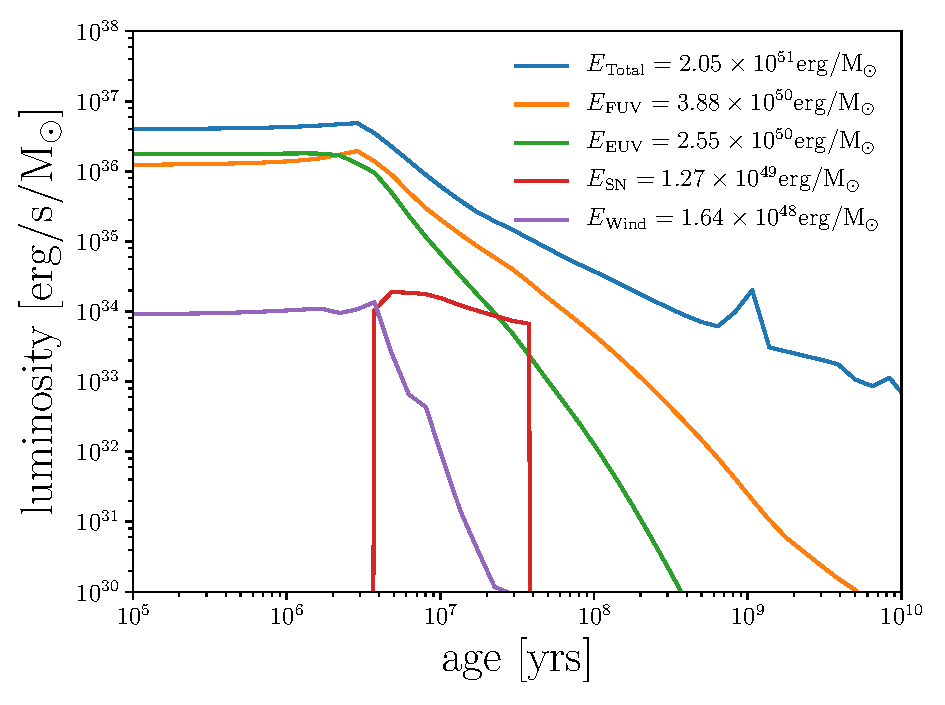
\includegraphics[width=1\linewidth]{Figures/uvsn.pdf}
\caption{Luminosity per solar mass as a function of time for a stellar 
population having a Chabrier initial mass function \citep{chabrier03}.}
\label{fig:uvsn}
\end{figure}

However, the way in which this massive output of UV radiation is deposited 
and consequently affects the interstellar medium (ISM) is still unclear. 
Attempts at numerically exploring these affects without the use of a full 
radiative transfer method have produced conflicting results. Simulations done
by \cite{gritschnederEt09} and \citep{walchEt12} suggest that ionizing feed 
back from large O-type stars before the first supernovae ($<1-3\rm{Myr}$) have 
a significant effect on star formation rate. Whereas \cite{daleEt12} 
conclude the affects on star formation rate to be small.

With that in mind it may then come as a surprise that RT has been treated 
rather poorly in most large scale astrophysical simulations, usually as some 
imposed uniform background. This is not because of carelessness or lack of 
effort, but because RT is an intrinsically complex and expensive problem. 
The complexity of this problem is firstly evident in the classical RT equation 
\citep[e.g.][]{mihalasMihalas84},
\begin{equation} \label{eqn:classicrt}
\left[ \frac{1}{c} \frac{\partial}{\partial t} + \mathbf{\hat{n} \cdot \nabla}
 \right] I\left(\mathbf{x}, \mathbf{\hat{n}}, t, \nu\right) = 
\epsilon\left(\mathbf{x}, \mathbf{\hat{n}}, t, \nu\right) - 
\alpha\left(\mathbf{x}, \mathbf{\hat{n}}, t, \nu\right) 
I\left(\mathbf{x}, \mathbf{\hat{n}}, t, \nu\right),
\end{equation} 
where $I$, $\epsilon$ and $\alpha$ are the intensity, emissivity and 
extinction coefficients respectively and all depend on position $\mathbf{x}$, 
unit direction of light propagation $\mathbf{\hat{n}}$, time $t$ and frequency 
$\nu$. Apart from being a seven dimensional problem, RT has the highest 
possible characteristic speed of $c$, the speed of light. Also, unlike a force 
at a distance problem such as gravity, RT depends on the properties of the 
intervening material which is handled by the extinction term, $\alpha$.

Because of this complexity, a na\"ive numerical solution to the RT problem 
scales with the number of resolution elements like $\bigO{N^{7/3}}$ and 
requires a timestep thousands of times smaller than typical courant times in 
astrophysics. This costly scaling is simply a result of the three major parts 
that go into computing the radiation field in a simulation. Firstly, a 
radiation field is represented by a simulation's $N$ resolution elements, so 
the field intensity needs to be computed at $N$ points in the simulation 
volume. Secondly, each resolution element's intensity value is made up of 
contributions from $\NS$ sources of radiation. This can also be thought of as 
$\NS$ rays of light being computed per resolution element. This leads to a 
scaling for the total number of rays computed in a simulation going as 
$\NR = N \times \NS$, which is $\bigO{N^2}$ assuming the $\NS = N$. This 
fact alone limits rudimentary RT methods to only small scale problems, such as 
ionization by a small handful of massive stars \citep{howard16, howard17}, to 
avoid $\bigO{N^2}$ scaling. Finally, each ray of light interacts with the 
medium along its path as mentioned earlier. Since the medium is represented by 
the simulation's $N$ resolution elements and $N$ is proportional to the 
simulation volume, a one dimensional ray intersects with $\bigO{N^{1/3}}$ 
resolution elements. Using the total number of resolution elements interacted 
with as a measure of computational cost we get that the computational cost is 
proportional to $N \times \NS \times N^{1/3}$, which is $\bigO{N^{7/3}}$. 
This poor scaling with resolution elements makes it unfeasible to simulate RT 
along with gravity and hydrodynamics methods that scale like $\bigO{N\log N}$. 
After breaking down the source of computational complexity in the RT problem 
it is evident that something needs to be done about the strong dependence on 
$\NS$ and the $N^{1/3}$ cost of computing each ray to attain a feasible RT 
method.

A feasible RT method would have to solve a simplified RT problem. The first 
one of these simplifications divides RT methods into two different categories 
based on how they treat $c$ in Eq. \ref{eqn:classicrt}. For methods that use a 
finite $c$, which is often a reduced speed of light, the partial time 
derivative remains in Eq. \ref{eqn:classicrt} and the radiation field 
is advected or ``evolved''. Methods that solve the RT equation in this way, 
which we will call evolutionary methods, include moment methods like OTVET 
\citep{gnedinAbel01} and  RAMESE-RT \citep{rosdahlTeyssier15} as well as 
photon packet propagation methods like TRAPHIC \citep{pawlikSchaye08}, SPHRAY 
\citep{altayEt08} and SimpleX2 \citep{paardekooperEt10}. On the other hand, in 
limit where $c$ is taken to be infinite, the partial time derivative in 
Eq. \ref{eqn:classicrt} goes to zero and the radiation field can be 
computed instantaneously as a computational geometry problem. Methods that 
solve the RT equation in this way, which we will refer to as instantaneous 
methods, include forward ray tracers such as $\rm C^2Ray$ 
\citep{mellemaEt06a}, Moray \citep{wiseAbel11} and Fervent 
\citep{baczynskiEt15} as well as reverse ray tracers such as TreeCol 
\citep{clarkEt12} and URCHIN \citep{altayTheuns13}. 

Instantaneous methods typically take the form of ray tracers. Ray tracers are 
the most simple, natural way to go about solving the RT problem. Forward ray 
tracers trace many rays outward from sources of radiation, similarly to the 
actual phenomena, in hope that they will intersect resolution elements for 
which the radiation field will be computed. As a result, a number of rays per 
source comparable to the number of resolution elements is needed to insure 
accuracy. Thus, na\"ive ray tracers scale with number of resolution elements 
like $\bigO{N \NS N^{1/3}}$. This scaling limits forward ray tracers to 
problems with few sources to avoid $\mathcal{O}(N^{7/3})$ like scaling. 
\comment{Wadsley: Note the bit about ray clumping not really saving 
the day because you still end up with O(N) ray segments and often a large 
multiplier (e.g. Abel \& Gnedin approach). Grond: Need some clarification on 
this point.}

Recently there has been some focus on reverse ray tracing methods by
\cite{clarkEt12} and \cite{altayTheuns13}. These methods are not general, 
as they specifically compute continuum radiation (from the post ionization UV 
background) and not from internal sources of radiation. However, the idea of 
reverse ray-tracing indroduces many advantages relative to reverse raytracing.
A main difference between forward and 
reverse ray tracing is that reverse ray tracers trace rays from the resolution 
elements directly to the sources of radiation. Tracing from the sinks 
guarantees the density distribution is well sampled near the resolution 
element as apposed to forward ray tracing where one would have to increase the 
number of rays per sink to guarantee this type of accuracy. Put simply, 
radiation is computed exactly where it is needed. This is especially 
advantageous in adaptive mesh and Lagrangian simulations such as smoothed 
particle hydrodynamics (SPH) simulations, as low density regions are 
represented by few resolution elements, and thus extra work is not done to 
resolve said regions. An added benefit to reverse ray tracing that adaptive 
time steps can be used. However, just performing a na\"ive reverse ray trace 
does not avoid $\bigO{N \NS N^{1/3}}$ scaling with resolution elements, and 
so the inability to model many sources remains the most significant barrier 
current instantaneous methods face when trying to solve the general RT 
problem. However, on any given substep $N_{\rm sink}$ can be dramatically 
reduced to be just the active sinks. In simulations with adaptive timesteps 
the active fraction on a given step is typically less than a percent of the 
total.

Evolutionary methods are typically based on evolving moments of the radiation 
field stored at each resolution element. They have no dependence on the number 
of sources, and scale like $\mathcal{O}(N)$ with the number of resolution 
elements, allowing them to handle large numbers of sources and scattering. 
Although evolutionary methods can handle both optically thin and thick 
regimes, they loose directional accuracy in intermediate regimes and suffer 
from directional accuracy in general.

Photon packet propagation methods, such as TRAPHIC \citep{pawlikSchaye08}, are 
an evolutionary approach that performs better in the optically thin regime. 
TRAPHIC introduces virtual particles (ViPs) to propagate their photon packets 
in less dense, optically thin regions lacking in SPH particles. 
They also preserve directionality quite well, however Monte Carlo aspects of 
how they propagate their photon packets introduce significant Poisson noise 
into their computed radiation field. Monte Carlo resampling is shown to reduce 
this noise but is quite expensive and deteriorates the initially sharp 
shadows. Both of these methods scale linearly with resolution elements as 
mentioned before, but are also forced to operate on every resolution element. 
In moment methods the radiation field for every grid cell needs to be 
computed, and in photon packet propagation methods the photon packets hop 
particle to particle. In the case of TRAPHIC, their $N$ is even greater than 
the number of SPH particles including the addition of ViPs. \comment{Wadsley: 
Need to discuss timestepping for evolutionary methods. Grond: Need some 
clarification.} Regardless, TRAPHIC is arguably the best general RT method due 
to its ability to handle both the optically thick and thin regimes with 
feasible scaling.

We hope from this introduction to the state of the art in RT methods it is 
apparent that there is room for improvement, especially in the area of 
instantaneous methods. Although promising work has been done with reverse ray 
tracers like TreeCol and URCHIN, a general implementation of one has yet to be 
developed and published. There is also the problem of scaling with radiation 
sources in instantaneous methods that reverse ray tracers alone do not solve. 
Therefore we have developed \acro{}, a $\bigO{N \log^2 N}$ reverse ray tracer 
designed to solve these problems and fill this niche. In Section 
\ref{sec:mthd} we detail the specific RT equations \acro{} solves 
(Subsection \ref{sec:rteq}) and the general \acro{} algorithm (Subsection 
\ref{sec:algo}) as well as specifics of our implementation in 
\textsc{Gasoline} (Subsection \ref{sec:specs}). In Section \ref{sec:tsts} we 
present a suite of tests demonstrating the algorithm's ability to accurately 
compute fluxes, ionization fronts and shadows in the optically thick and thin 
regimes. These tests also allow us to explore how \acro{}'s accuracy criteria 
predicts error and affects computation cost. The computational cost is bounded 
and characterized in a general case to substantiate the $\bigO{N \log^2 N}$ 
claim made earlier. Finally, in Section \ref{sec:disc} we discuss \acro{}'s 
strengths and shortcomings and conclude how they enable and constrain the 
types of problems \acro{} can handle. We will also discuss apparent 
improvements that can be made in the future in this section.

\section{Method}\label{sec:mthd}
\subsection{Simplifications to the full RT problem}\label{sec:rteq}
Before describing \acro{}, let's first define the 
simplified version of the classical RT equation the method solves. Since 
\acro{} is an instantaneous method, $c$ is set to infinity eliminating the 
partial time derivative in \ref{eqn:classicrt} leaving us with the 
instantaneous RT equation,
\begin{equation} \label{infcrt}
\mathbf{\hat{n} \cdot \nabla} I\left(\mathbf{x}, \mathbf{\hat{n}}, t, 
\nu\right) = \epsilon\left(\mathbf{x}, \mathbf{\hat{n}}, t, \nu\right) - 
\alpha\left(\mathbf{x}, \mathbf{\hat{n}}, t, \nu\right) 
I\left(\mathbf{x}, \mathbf{\hat{n}}, t, \nu\right).
\end{equation}
The emissivity term in the above equation, $\epsilon$, describes a continuous 
emitting medium. \acro{} assumes sources of radiation are continuous, but 
being a numerical method it needs to represent sources of radiation as 
discrete resolution elements. In this case $\epsilon$ is a sum of delta 
functions and the solution to the RT equation becomes a linear combination of 
contributions from all sources of radiation. Also, since we are considering 
sources one by one we can start using the path length $s$ between a source and 
resolution element as our integration element
\begin{equation}
\label{eqn:combtransfer}
\frac{dI}{ds} = -\alpha I.
\end{equation}
We can then combine the path length and extinction coefficient to solve for 
intensity by integrating 
\begin{equation}
\label{eqn:dtau}
d\tau = \kappa \rho ds, 
\end{equation}
the optical depth, where $\kappa$ is opacity and $\rho$ is density. This 
leaves us with
\begin{equation}
\label{eqn:absorbtransfer}
\frac{dI}{d\tau} = -I,
\end{equation}
the final version of the RT problem this method solves. The solution to this 
equation is 
\begin{equation}
\label{eqn:ient}
I(s) = I(s_0)e^{-\tau(s)},
\end{equation}
where $I(s_0)$ is the intensity of the source and $\tau(s)$ is the only
quantity to be integrated in our method
\begin{equation}
\label{eqn:tauint}
\tau(s) = \int_{s_0}^s \kappa(s) \rho(s) ds.
\end{equation}
\comment{Wadsley: This is a bit out of the blue. You just skipped from one 
source to all of them without saying you did that. Grond: I'm a bit stuck on 
this.}

We can use the radiation intensity directly in heating, chemistry and 
ionization functions which are typically a function the total intensity from 
all radiation sources. We can then take moments of the intensity to obtain 
useful quantities such as radiation flux 
\begin{equation}
\label{eqn:flux}
\mathbf{F} = \int I cos\theta d\Omega \mathbf{\hat{n}},
\end{equation}
and radiation pressure
\begin{equation}
\label{eqn:pressure}
\mathbf{p} = \frac{1}{c}\int I cos^2\theta d\Omega \mathbf{\hat{n}}.
\end{equation}
\comment{Wadsley: What is dOmega -- where did the integrals come from? Grond: 
Rybicki and Lightman. Wadsley: It might be clearer if you said, ``for point 
sources the contribution is I delta(theta)'' or something like that. Grond: 
Need some clarification here.}
Because we assume our sources of radiation to be true point sources, 
$cos\theta = 1$. If the angular size of a resolution element relative to the 
source of radiation is small enough such that the small angle approximation 
holds true, it should also hold that there is a one-to-one correspondence 
between intensity and flux. Thus, flux from a \textit{single} source can be 
written simply as 
\begin{equation}
\label{eqn:simpflux}
\mathbf{F} = I(s_0)e^{-\tau(s)} \mathbf{\hat{n}} = \frac{L}{4\pi s^2}
e^{-\tau(s)} \mathbf{\hat{n}},
\end{equation}
where $L$ is the luminosity of the source of radiation. The total flux is then 
computed by summing up flux contributions from all sources. For the remainder 
of paper we represent the radiation field as flux values computed via the 
above expression. 

\subsection{Algorithm}\label{sec:algo}
Please note that although \acro{} has been initially implemented in the 
SPH code \textsc{Gasoline} \citep{wadsleyEt03}, \acro{} is not specific to 
\textsc{Gasoline} or SPH in general. The method only requires that the 
simulation volume is hierarchically partitioned in space and so it could be 
used directly in an adaptive mesh refinement (AMR) code.
 
\begin{figure*}
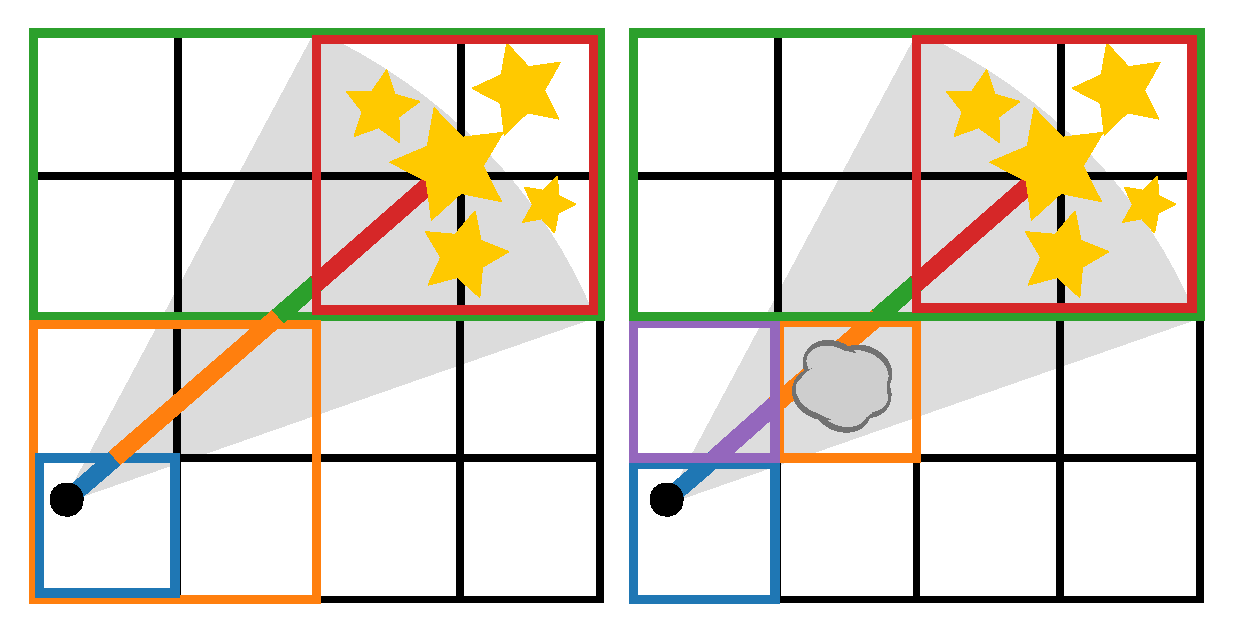
\includegraphics[width=1\linewidth]{Figures/algorithm.pdf}
\caption{}
\label{fig:algorithm}
\end{figure*}
The \acro{} algorithm is based around a tree data structure which partitions 
the simulation volume hierarchically in space. The smallest resolution 
elements are or are contained by in the leaf nodes of the tree data structure. 
In Lagrangian or ``particle'' methods such as SPH, a number of SPH particles 
can be contained by a leaf node or ``bucket''. The maximum number of particles 
per bucket is referred to as $N_B$. In Eulerian or ``grid'' based methods the 
bucket is the smallest grid cell itself, so $N_B$ is effectively one. $N$ 
resolution elements hold radiation intensity values and represent the 
radiation field \acro{} computes. 

\subsubsection{Source Merging}
As mentioned in the introduction, a na\"ive algorithm would compute 
interactions between a resolution element and  all sources of radiation. If we 
assume the number of resolution elements is equal to the number of sources, 
an infeasible number of interactions would need to be computed, scaling like 
$\bigO{N^2}$. To mitigate this $N^2$ scaling \acro{} employs source merging 
similar to particle merging in the \cite{barnesHut86} tree-based gravity 
solver which has remained commonplace in astrophysical simulations 
\citep{benz88,vineSigurdsson98,springelEt01,wadsleyEt03,hubberEt11}. Merging 
sources of radiation was first implemented in a rudimentary version of \acro{} 
that did not consider extinction of any kind \citep{kannanEt14}. Sources of 
radiation are merged together at their centre of luminosity if they meet an 
``opening angle'' criteria. This criteria is defined as 
\begin{equation}
\label{eqn:openangle}
\tO > l/r,
\end{equation}
where $l$ is the side length of a tree cell, $r$ is the distance between the 
centre of luminosity of a source and centre of mass of a resolution element 
and $\tO$ is the opening angle, a fixed accuracy parameter. If a 
group of sources occupy the biggest tree cell that meets this criteria, all 
sources in that cell are merged into one, considerably reducing the number of 
interactions \acro{} computes. This is illustrated in the left panel of Fig. 
\ref{fig:algorithm}, where the grey angle represents a cell whose angular size 
meets the opening angle criterion.

The cost savings of source merging can be quantified by integrating the number 
of tree cells that are ``opened'' according to the opening angle criteria. 
These opened cells will have their sources merged making them a single source. 
We will call the total count of the opened cells $N_{\rm open}$. We can 
theoretically compute $N_{\rm open}$ this by integrating spherical shells of 
thickness $dr$ along the path from a resolution element $r$, and then dividing 
the sphere volume by the volume of an opened cell, $V_{\rm open}(r)$.
\begin{equation}
\label{eqn:nsint}
N_{\rm open} = \int_{R_0}^R \frac{4\pi r^2}{V_{\rm open}(r)} dr
\end{equation}
The bounds of the above integral go from $R_0$, the size of a bucket 
cell, to $R$, the length of the simulation volume. Because the number of 
particles in a simulation is proportional to the simulation volume, the 
lower integration limit can be expressed using particle numbers via 
\begin{equation}
\label{eqn:ratio}
\frac{R_0}{R} = \sqrt[3]{\frac{N_B}{N}},
\end{equation} 
the cubed root of the ratio of the average number of particles per bucket, 
$N_B$, to the total number of simulation particles. Note that $N_B$ 
($N_B = 10$ for this paper) is only needed for particle methods. In a grid 
method a bucket is just the lowest level grid cell in the tree and $N_B=1$. 
The opened cell volume can also be rewritten by cubing the opening angle 
criteria
\begin{equation}
\label{eqn:vcell}
V_{\rm open}(r) = l^3 = \tO^3 r^3.
\end{equation}
Substituting gives us the following integral and its solution,
\begin{equation}
\label{eqn:nssoln}
N_{\rm open} = \int_{\left(\frac{N}{N_B}\right)^{-\frac{1}{3}}}^R 
\frac{4\pi r^2}{\tO^3} dr
\sim \log{N/N_B}.
\end{equation}
This result means that the number of interactions scales like 
$\bigO{N \log N}$. This is also the total cost scaling in the optically 
thin regime, which is unsurprising given the RT problem is almost identical to 
the gravity problem in the absence of intervening material. That brings up the 
next part of the algorithm, what to do about tracing a ray in the optically 
thick regime.

\subsubsection{Tracing Rays}
In the presence of absorbing material along a ray, the optical depth needs to 
be computed along said ray by computing the optical depth integral introduced 
in Eq. \ref{eqn:tauint}. To solve this integral numerically, we traverse the 
tree between the source and resolution element to build up the optical depth. 
This is possible because the tree partitions and fills space, thus all the 
intervening material should be contained in the tree we traverse. Making use 
of properties computed during the tree build, we can compute the optical depth 
of the $i$'th piece of the ray ($\tau_i$) using the intersection length 
of the cell and ray ($s_i$) as well as the average density ($\bar{\rho}_i$) 
and average opacity ($\bar{\kappa}_i$) in the cell
\begin{equation}
\label{eqn:taui}
\tau_i = \bar{\rho}_i \bar{\kappa}_i s_i.
\end{equation}
The total optical depth is then summed up during the tree walk,
\begin{equation}
\label{eqn:tausum}
\tau = \sum_i \tau_i,
\end{equation}
giving us everything needed to evaluate Equation \ref{eqn:simpflux}. 

This process is also illustrated in the left panel of Figure 
\ref{fig:algorithm}. In this figure ray segments and corresponding cells share 
the same colour. When referring to specific cell colours, they will also be 
identified by two sets of points $[(x,y),(x,y)]$ corresponding to the bottom 
left and top right vertices of the cell respectively. Dotted lines are used to 
distinguish consecutive ray segments and help associate ray segments and their 
corresponding cells. In the left panel of Figure \ref{fig:algorithm} there are 
two important things to note. Firstly, since we are performing a reverse ray 
trace, the resolution element denoted by the black circle is intrinsically 
well resolved at the bucket cell (the blue cell at at $[(0,0),(1,1)]$) level. 
However, the second point is that as the tree is walked upwards space becomes 
less resolved. It should be apparent that the central parts of the ray are 
less resolved (the green cell at $[(0,2),(4,4)]$) and as you move towards the 
source or resolution element the ray becomes more resolved (the red cell at 
$[(2,2),(4,4)]$ and the orange cell $[(0,0),(2,2)]$). This can be looked at in 
two ways. If the medium is uniform, the algorithm can be extremely efficient 
while still being able to resolve a sharp feature in the radiation field such 
as an ionization front. However, if the medium is highly irregular along the 
ray the algorithm will not be able to resolve sharp density and opacity 
gradients which could significantly alter the optical depth. Thus adaptive 
refinement is needed during the tree walk to accurately resolve the medium 
along the ray.

\subsubsection{Adaptive Refinement}
Consider the right panel in Figure \ref{fig:algorithm}. A dense blob of gas 
to be resolved resides in the orange highlighted cell at $[(1,1),(2,2)]$. At 
the point in the tree walk where we reach the orange highlighted cell at 
$[(0,0),(2,2)]$ in the left panel, a decision needs to be made on whether the 
current cell sufficiently represents the media. This decision is made by a 
refinement criteria. If the cell passes the criteria to refine, rather than 
using its average properties we recursively check the cell's children until 
the criteria fails. Thus building a better resolved section of the ray. 

Difficulty comes in choosing a refinement criteria that is both accurate and 
efficient. Ideally, the criteria should be true when an average optical depth 
in a region may not be accurate to the true distribution, such as a clumpy 
medium where the average density and opacity is much higher than the 
``effective'' density and opacity \citep{varosiDwek99, hegmanKegel03}. For 
this reason we have chosen an optical depth based refinement criteria that is 
unique to \acro{}.

\begin{figure}
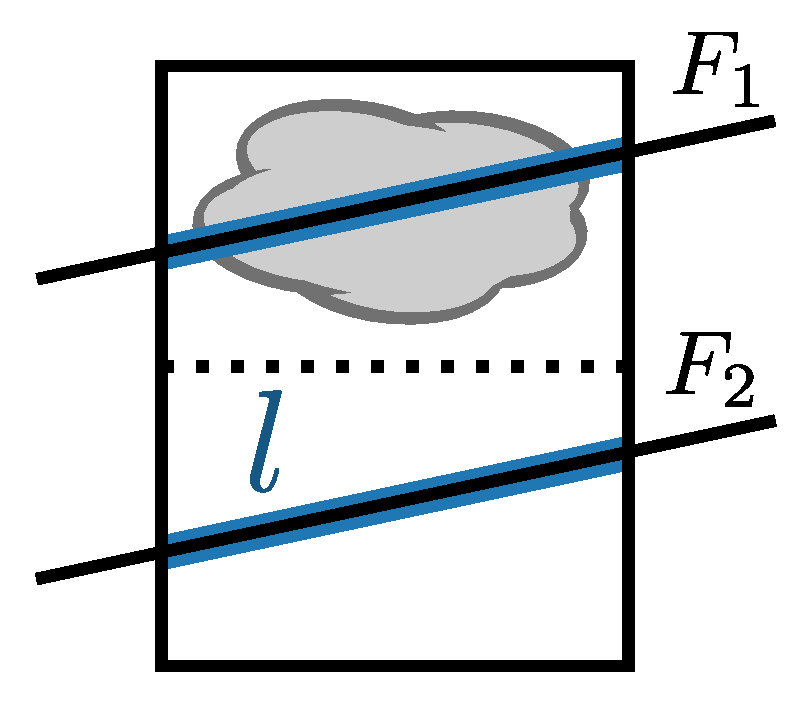
\includegraphics[width=1\linewidth]{Figures/refine.pdf}
\caption{}
\label{fig:refine}
\end{figure}
Consider two rays through through a large cell as in Figure \ref{fig:refine}. 
These rays represent what the case would be if properties of the children were 
used instead of the parent cell. We can compute the minimum and maximum 
absorption coefficients $\alpha_{\rm min}$ and $\alpha_{\rm max}$, via their 
minimum and maximum density and opacity values computed during the tree build. 
This multiplied by the intersection length $l$ gives us the minimum and 
maximum optical depths, $\tau_{\rm min}$ and $\tau_{\rm max}$. We can then 
test the following refinement criteria
\begin{equation}
\label{eqn:refcrit}
\tr < \tau_{\rm max} - \tau_{\rm min},
\end{equation}
and refine if it is true. The fractional error in flux, per ray segment, for a 
chosen value of $\tr$ is
\begin{equation}
\label{eqn:reffrac}
\frac{F_1 - F_2}{F_1} \leq 1 - e^{-\tau_{\rm max}-\tau_{\rm max}} 
\lesssim \tr,
\end{equation}
for small $\tau$, making the refinement criteria a convenient choice of 
parameter for controlling error.

If the refinement criteria passes at the bucket level, individual particles 
within a bucket are considered. A straight forward $N^2$ ray tracing scheme 
similar to SPHRay \citep{altayEt08} can be performed on bucket particles and 
their neighbours. In the worst case where the refinement criteria passes the 
bucket level every time, a cost of $\bigO{C_n N}$ is added to the scaling, 
where $C_n$ is the constant number of SPH neighbours.

Fully characterizing the computational cost of the algorithm including the 
addition of adaptive refinement follows the same method as used earlier. 
However, now instead of integrating the number of sources we integrate the 
total number of ray segments computed. We will look at two cases, not refining 
at all and fully refining down to the bucket level. This will give us upper 
and lower bound for the algorithms scaling as characterizing the refinement 
between these extremes depends on the specific density and opacity 
distributions being operated on.

First let's consider the case where the refinement criteria always passes and 
all rays are resolved down to the bucket level. The number of segments per ray 
is then just the length of a ray divided by the size of a bucket. We can 
express this as
\begin{equation}
\label{eqn:nseg}
N_{\rm seg} = \frac{r}{R_0} = \frac{r}{R}\left(\frac{N}{N_B}\right)^\frac{1}{3}
\end{equation}
after substituting Eq. \ref{eqn:ratio} in for $R_0$. Since $\NS$ is also the 
number of rays computed, the total number of ray segments computed is just Eq. 
\ref{eqn:nsint} multiplied by the number of ray segments
\begin{equation}
\label{eqn:nsegint}
N_{\rm seg} = \int_{\left(\frac{N}{N_B}\right)^{-\frac{1}{3}}}^R 
\frac{4\pi r^2}{\tO^3}
\frac{r}{R}\left(\frac{N}{N_B}\right)^\frac{1}{3} dr
\sim N(2N/N_B)^\frac{1}{3}.
\end{equation}
This results means that the total cost of the algorithm scales like 
$\bigO{N^{4/3}}$ in the worst case.

In the case were the refinement criteria never passes, the ray is split into 
segments made up of the cells traversed in the tree walk of the sub-tree going 
from source to resolution element. The number of cells traversed in a tree walk
is equal to the logarithm of the number of leaf nodes contained within the 
sub-tree. The number of leaf nodes in the sub-tree is also given by Eq. 
\ref{eqn:nseg}, so by taking the logarithm of Eq.\ref{eqn:nseg} and adding two 
for the two buckets on eiter side of the sub-tree we come to
\begin{equation}
\label{eqn:nseg2}
N_{\rm seg} = \log_2\left[\frac{r}{R}\left(
\frac{N}{N_B}\right)^\frac{1}{3}\right],
\end{equation}
where the logarithm is base two as \textsc{Gasoline} and thus \acro{} is 
implemented using a binary tree. As before we multiply Eq. \ref{eqn:nsint} 
by the number of ray segments and integrate the following
\begin{equation}
\label{eqn:nsegint2}
N_{\rm seg} = \int_{\left(\frac{N}{N_B}\right)^{-\frac{1}{3}}}^R 
\frac{4\pi r^2}{\tO^3}
\log_2\left[\frac{r}{R}\left(
\frac{N}{N_B}\right)^\frac{1}{3}\right] dr
\sim N\log^2(128 N/N_B).
\end{equation}
This results means that the total cost of the algorithm scales like 
$\bigO{N\log^2N}$ in the best case.

\subsubsection{Background Radiation}
In order to treat simulations properly we must account for the radiation 
coming from the rest of the universe outside of the simulation volume. Most 
current codes apply a constant UV field to the entire box, essentially the 
lowest order approximation possible. Some specialized codes like URCHIN 
\citep{altayTheuns13} do a reverse ray trace to the edge of the box, where the 
background flux is assumed to be coming from. Others, such as TRAPHIC 
\citep{pawlikSchaye08} allow their ray trace to be periodic. We believe
that this periodic treatment is problematic. The cosmic UV radiation field 
originates from very large distances on the order of a gigaparsec. This is too 
large of a region to practically simulate, so radiation originating from 
periodicity is too local.

Instead, we have implemented a method involving tracing ``background sources'' 
similar to URCHIN. ``Background'' particles are distributed in a spiral 
pattern on the surface of a sphere at the very edge of the simulation volume 
(or at a large distance if required) and the number of sources can be varied 
to match the required angular resolution of the background. Finding the flux 
at the centre of a sphere of sources is a problem akin to Newton's Shell 
Theorem. However, because the intensity does not cancel like force, the 
solution differs and is as follows:
\begin{equation}
\label{eqn:cosmof}
F(r) = \frac{L}{8\pi R} \ln \left(\frac{R+r}{R-r}\right),
\end{equation}
where $L$ is the total luminosity of the emitting shell, $R$ is the radius of 
the sphere and $r$ is the radius the flux is being computed at. The shape of 
the function can be seen in Figure \ref{fig:cosmof} where we have plotted the 
flux as a function of radius for a homogeneous, optically thin test volume.
\begin{figure}
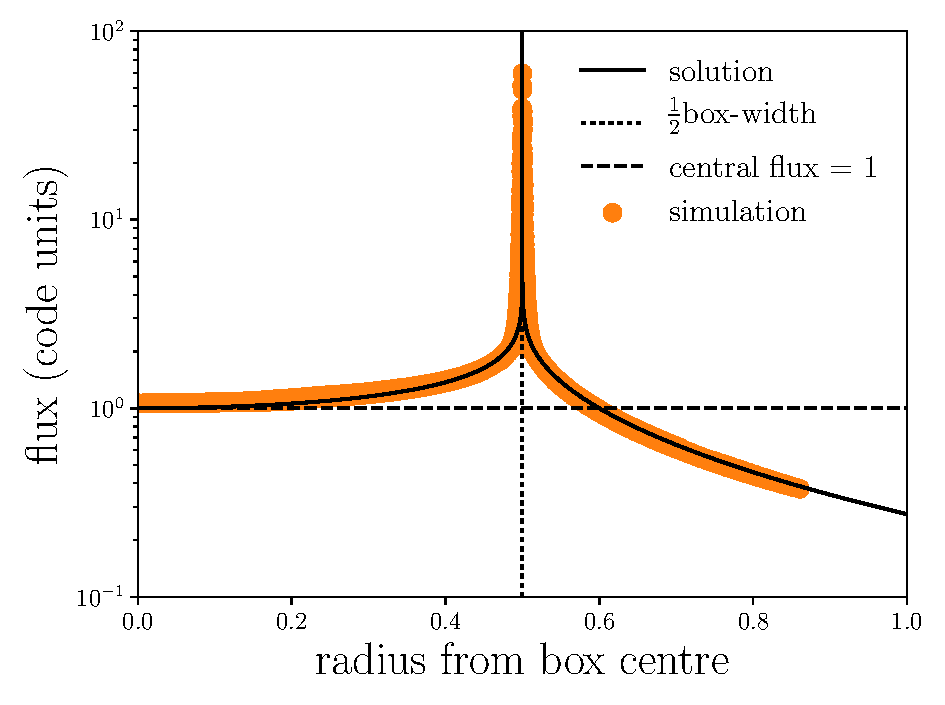
\includegraphics[width=1\linewidth]{Figures/cosmofield.pdf}
\caption{}
\label{fig:cosmof}
\end{figure}

Note that due to the logarithm in Equation \ref{eqn:cosmof}, the flux is 
nearly constant at small radii. Since most cosmological zoom in simulations 
only consider gas at a fairly small radius, this setup of background sources 
is an acceptable method to provide a background flux. A benefit of this method 
is that we can use all of the existing machinery described in the methods 
section, and only have to add temporary background star particles as the 
source of the background radiation. Also not that the simulation flux is over 
estimated near the central region and underestimated at large radii. When 
merging background sources which are all located on the surface of a sphere, 
the merged centre of luminosity will always be at a smaller radius than that 
the sphere radius. This can be remedied by enforcing merged background sources 
to always be located on the sphere. 

\subsection{Implementation Specifics}\label{sec:specs}
As mentioned earlier, \acro{} is not specific to either \textsc{Gasoline} or 
SPH.  However, in this subsection we would like to take the time to briefly  
introduce \textsc{Gasoline} and the specifics of \acro{}'s implementation in 
\textsc{Gasoline}.

\textsc{Gasoline} is a parallel smoothed particle hydrodynamics code for 
computing hydrodynamics and self-gravity in astrophysics simulations. It 
employs a 

In the current version of \acro{}, a separate tree is built for computing
radiative transfer. For development this is a convenient choice, but adds
extra cost and in the future a ``one tree to rule them all'' approach should
be adopted. The radiation tree inherits it's binary cell splitting from the
main tree in \textsc{Gasoline}. On of the main differences between these trees
is that the radiation tree is required to fill all space to enable, whereas
the main tree ``squeezes'' cell bounds to the furthest extents of an
particle's influence. This does not work in the context of RT as cell and ray
intersections need to be computed to sum up a correct optical depth.

\section{Code Tests}\label{sec:tsts}
\subsection{Sinusoidally Perturbed Glass}
\subsubsection{Initial Conditions}
To test the accuracy and general scaling of the algorithm, an varying initial 
condition (IC) that the accuracy criterion can operate on while being 
representative of a typical use case is needed. For this we have created a 
novel IC comprised of a unit length glass of $N$ SPH gas and $N$ star 
particles whose positions have been perturbed by 24 random sinusoidal modes. 
The initial glass of particles comes from as $16^3$ glass used to create 
initial conditions for other tests of \textsc{Gasoline} \citep{wadsleyEt17}. 
The total mass of gas particles is one, and the opacity of each particle is 
also one. This results in an optical depth across the width of the box of 
$\sim$1, making the simulation volume optically thin overall with dense, 
optically thick filamentary structure and underdense voids qualitatively 
similar to the cosmic web. Each star particle is also assigned a luminosity of 
one. A slice of this density distribution is plotted in Figure 
\ref{fig:sine_rho}. Appendix \ref{sec:icnd} contains a detailed explanation of 
how this IC was created including a table of modes used.
\begin{figure}
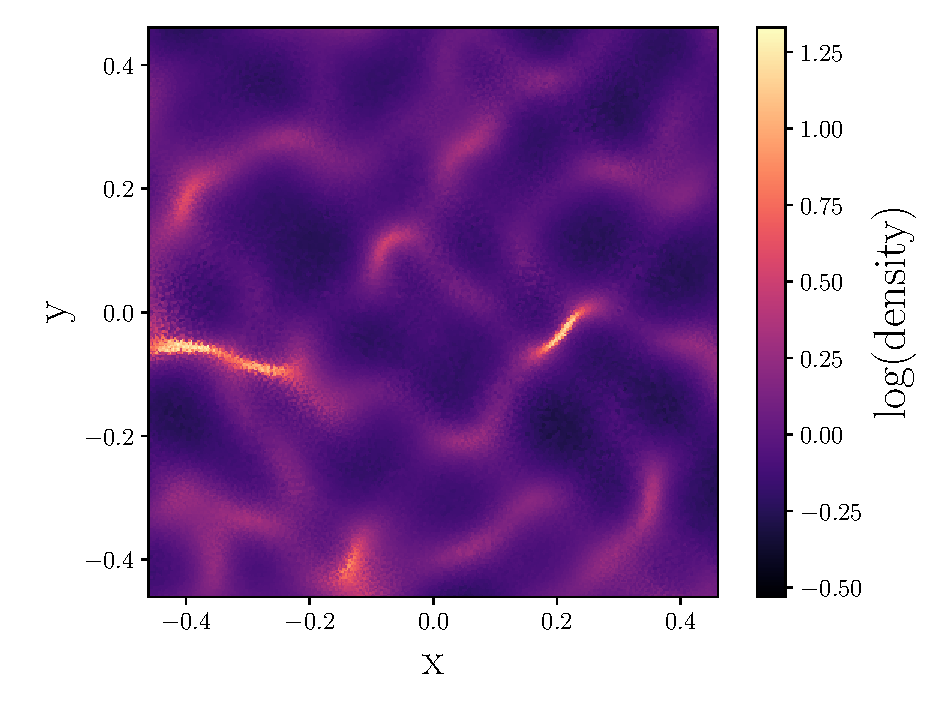
\includegraphics[width=1\linewidth]{Figures/sine_rho.pdf}
\caption{}
\label{fig:sine_rho}
\end{figure}

\subsubsection{Opening Angle}
The opening angle criteria's affect on accuracy and cost was tested by 
simulating the optically thin, sinusoidally perturbed glass IC with $\tO$ 
varying between 0 and 1. The results of this test are plotted in Figure 
\ref{fig:openangle}. The measure of cost is plotted as the total number of 
rays, $N_{\rm rays}$, computed per resolution element on the left $y$-axis. 
The number of rays is equivalent to the number of radiation sink-source 
interactions computed in a simulation time step. Using rays as a measure of 
cost allows us to separate the affects of the refinement criteria on cost. On 
the right $y$-axis, the root mean squared (RMS) fractional error relative to 
the radiation field computed with $\tO=0$. A refinement criteria 
value of $\tr = 0.1$ and $N=64^3$ for both star and gas particles.
\begin{figure}
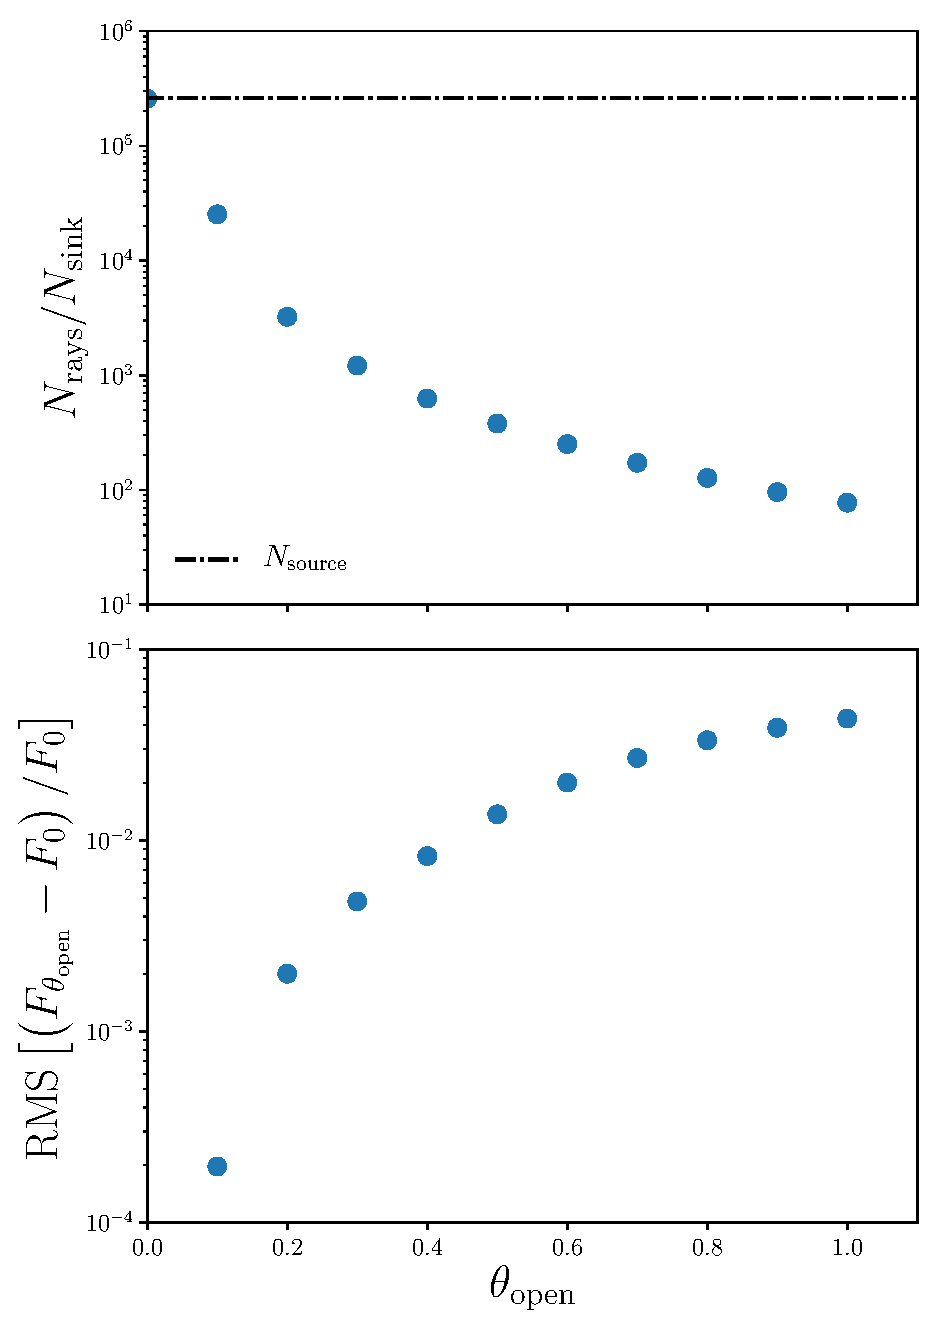
\includegraphics[width=1\linewidth]{Figures/opening_angle.pdf}
\caption{}
\label{fig:openangle}
\end{figure}

At $\tO=0.75$, the value used in all other tests and the 
default value for $\tO$ in many gravity solvers, 200 rays are 
computed per resolution element with an RMS fractional error of 3\%. To get to 
an RMS fractional error of about 1\%, a opening angle of $\tO=0.45$ is needed 
and costs only 500 rays per resolution element. The cost at 
$\tO=0.45$ is still much less than interacting with all $64^3$ 
($2.6\e{5}$) sources, and could be a standard default value to move forward 
with.

\subsubsection{Refinement Criteria}
Testing the refinement criteria is similar to testing the opening angle 
criteria. Again, the sinusoidally perturbed glass IC was simulated but now with 
a varying $\tr$ value. The results of this test are plotted in 
\ref{fig:refcrit}. The min and max values of $\tr$ tested were 
chosen such that the cost curve flattens out on either side. The left  hand 
side being where refinement has occurred down to the bucket level, and the 
right hand side end being where refinement is never done. 
A opening angle of 0.75 was used and $N=64^3$ for both star and gas particles. 
Cost is plotted on the left $y$-axis and RMS fractional error on the right 
$y$-axis. The measure of cost is now number of ray segments per resolution 
element, since the refinement criteria controls how refined a ray becomes. 
The measure of accuracy is again the RMS fractional error, but now relative to 
the radiation field computed with $\tr=1\e{-8}$, the lowest $\tr$ tested.
\begin{figure}
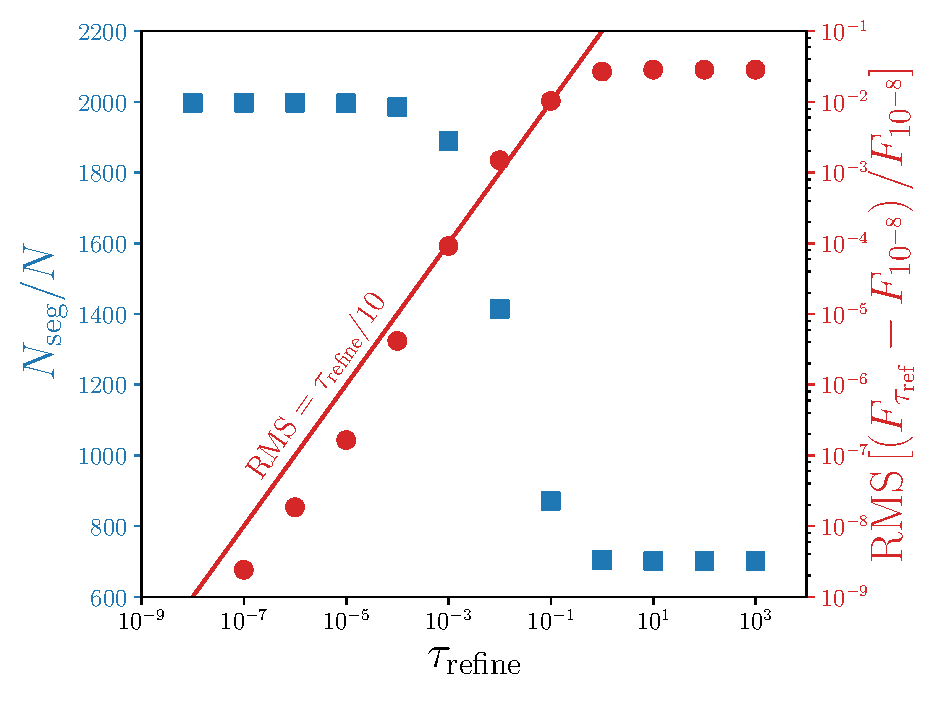
\includegraphics[width=1\linewidth]{Figures/refinement_criteria.pdf}
\caption{}
\label{fig:refcrit}
\end{figure}

At $\tr=0.1$, 1\% RMS fractional error is achieved with a cost of 
approximately 850 ray segments computed per resolution element, less than half 
the cost of refining all the way to the bucket level. Note also that RMS 
fractional error as a function of $\tr$ behaves predictably, lying below the 
RMS = $\tr$ line and roughly following the RMS = $\tr/10$ line plotted in 
Figure \ref{fig:refcrit}. This in in agreement with our theoretical claim in 
Equation \ref{eqn:reffrac}, that the maximum allowable error in flux per ray 
segment should be less than and proportional to $\tr$ for small $\tau$. 

The RMS fractional error maxes out at 2-3\% in this test. In this particular 
implementation of \acro{}, the walk along the ray goes up from both the bucket 
where the radiation sink resides and the opened cell where the source resides 
to the top of the tree. This built in level of refinement is the reason for 
the low maximum error. Other implementations, that walk the ray top down or up 
and then back down the tree, would need to rely more or solely on the 
refinement criteria. In principle, such a method could perform better than 
$\bigO{N\log^2 N}$.

\subsubsection{Scaling}
\begin{figure}
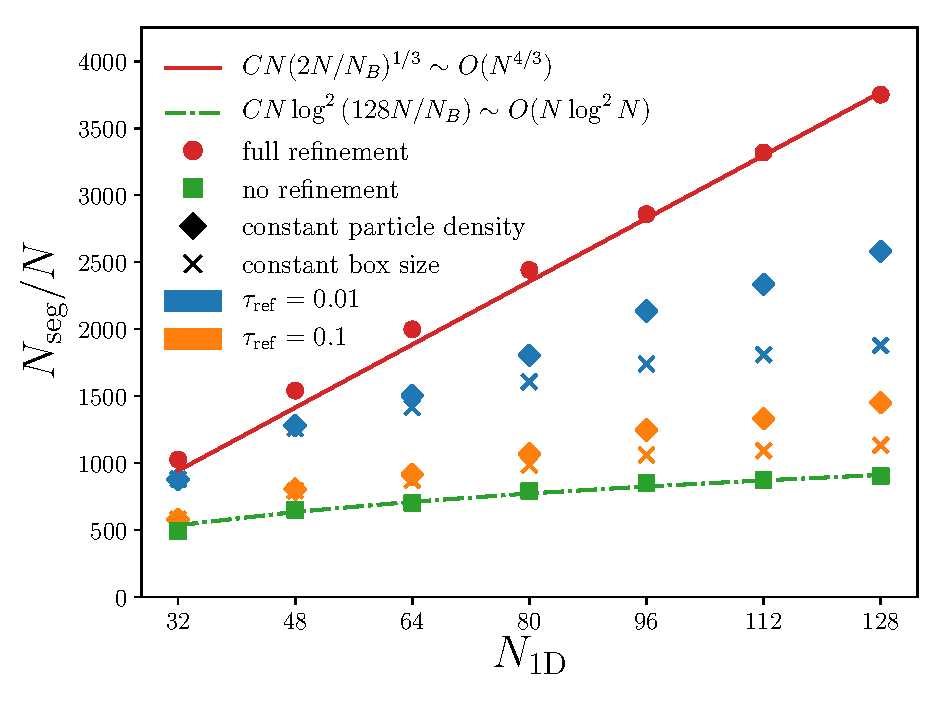
\includegraphics[width=1\linewidth]{Figures/particle_scaling.pdf}
\caption{}
\label{fig:pscale}
\end{figure}
To test cost scaling as a function of $N$, we hold $\tO$ constant at 0.75 and
vary $N$ between $32^3$ and $128^3$ in steps of $N_{\rm 1D} = 16$ for both gas 
and star particles. To substantiate our best and worst case theoretical 
scaling claims made in Equations \ref{eqn:nsegint2} and \ref{eqn:nsegint} 
respectively, the sinusoidally perturbed glass IC was simulated with $\tr=1\e 6$ 
to insure refinement was never performed and with $\tr=0$ to insure refinement 
was always performed down to the bucket level. Data from theses tests and 
fitted theoretical lines were plotted in Figure \ref{fig:pscale} and 
correspond very closely to each other. Note that the only parameter used to 
fit the theoretical lines from was a constant factor of $C$ placed in front of 
Equations \ref{eqn:nsegint} and \ref{eqn:nsegint2}.

Scaling behavior between the upper and lower limits was probed in two ways. 
Firstly, simulations were run with $\tr$ values of 0.1 and 0.01. Secondly, 
strong and weak scaling cases were simulated. The strong scaling case being 
where the box size was held constant and particle number increased. This is 
analogous to increasing the resolution of an isolated galaxy simulation. The 
weak scaling case is the opposite, where the box size is increased and 
particle density is held constant. This is analogous to simulating larger and 
larger cosmological boxes to achieve larger statistical samples. 

Again, data from these tests was plotted in Figure \ref{fig:pscale} where 
there are two interesting things to note. Firstly, the strong scaling case, 
which is typically the harder case to scale well in, scales better than the 
weak scaling case. The strong scaling data turns over more similarly to the
$N\log^2{N}$ function and costs less than the weak scaling data. This is 
because unlike gravity, tracing a ray through intervening material will always 
cost more on longer length scales. Whereas in the strong scaling case, an 
increased number of particles represent the same density and opacity 
distribution and the refinement criteria will still act in the similar way, 
now with more particles per cell to average over. The second thing to note is 
that the strong scaling case at $\tr=0.1$, which achieved an RMS fractional 
error of 1\% in the $N=64^3$ sinusoidally perturbed glass test, scales 
similarly to the no refinement data and fit to $N\log^2{N}$. 

\subsection{Isothermal Spheres}
\subsubsection{Initial Conditions}
The sinusoidally perturbed glass IC tested a generally optically thin, smooth 
density distribution. This is a good proxy for many astrophysical cases of 
interest, such as late stage galaxy evolution..As a test of how \acro{}'s 
refinement criteria can handle compact, optically thick features we created 
the Isothermal Spheres IC. This IC consists a single radiation source 
positioned in the top left corner and four spheres with $1/r^2$ density 
profiles embedded in a uniform glass. The spheres produce shadows down and to 
the right of the source. Accurate shadows can only be cast if the sharply 
peaked spheres are resolved correctly by the refinement criteria. Error 
specifically in the optically thick regime can be separated out by looking at 
only particles in shadow. The four isothermal spheres follow the density 
distribution described by
\begin{equation}
\rho(r) = \frac{\rho_0 \epsilon}{r^2 + \epsilon^2},
\end{equation}
where the softening length, $\epsilon$, is 0.002 and the central density, 
$\rho_0$, is 626. The IC was made by adding SPH gas particles near the 
sphere centers using a stretched glass of. \comment{Grond: James, could you 
fill this part in? I don't have the script you used to do this on hand.} These 
parameters set the maximum optical depth through a sphere to 
$\tau_{\rm max}=4$ (98\% reduction in flux) and the density at the edge of the 
spheres to one, matching the unit density of the uniform background. The 
isothermal spheres have a radius of 0.05 and are denoted by the grey circles 
in Figure \ref{fig:cellplot}.  
\begin{figure*}
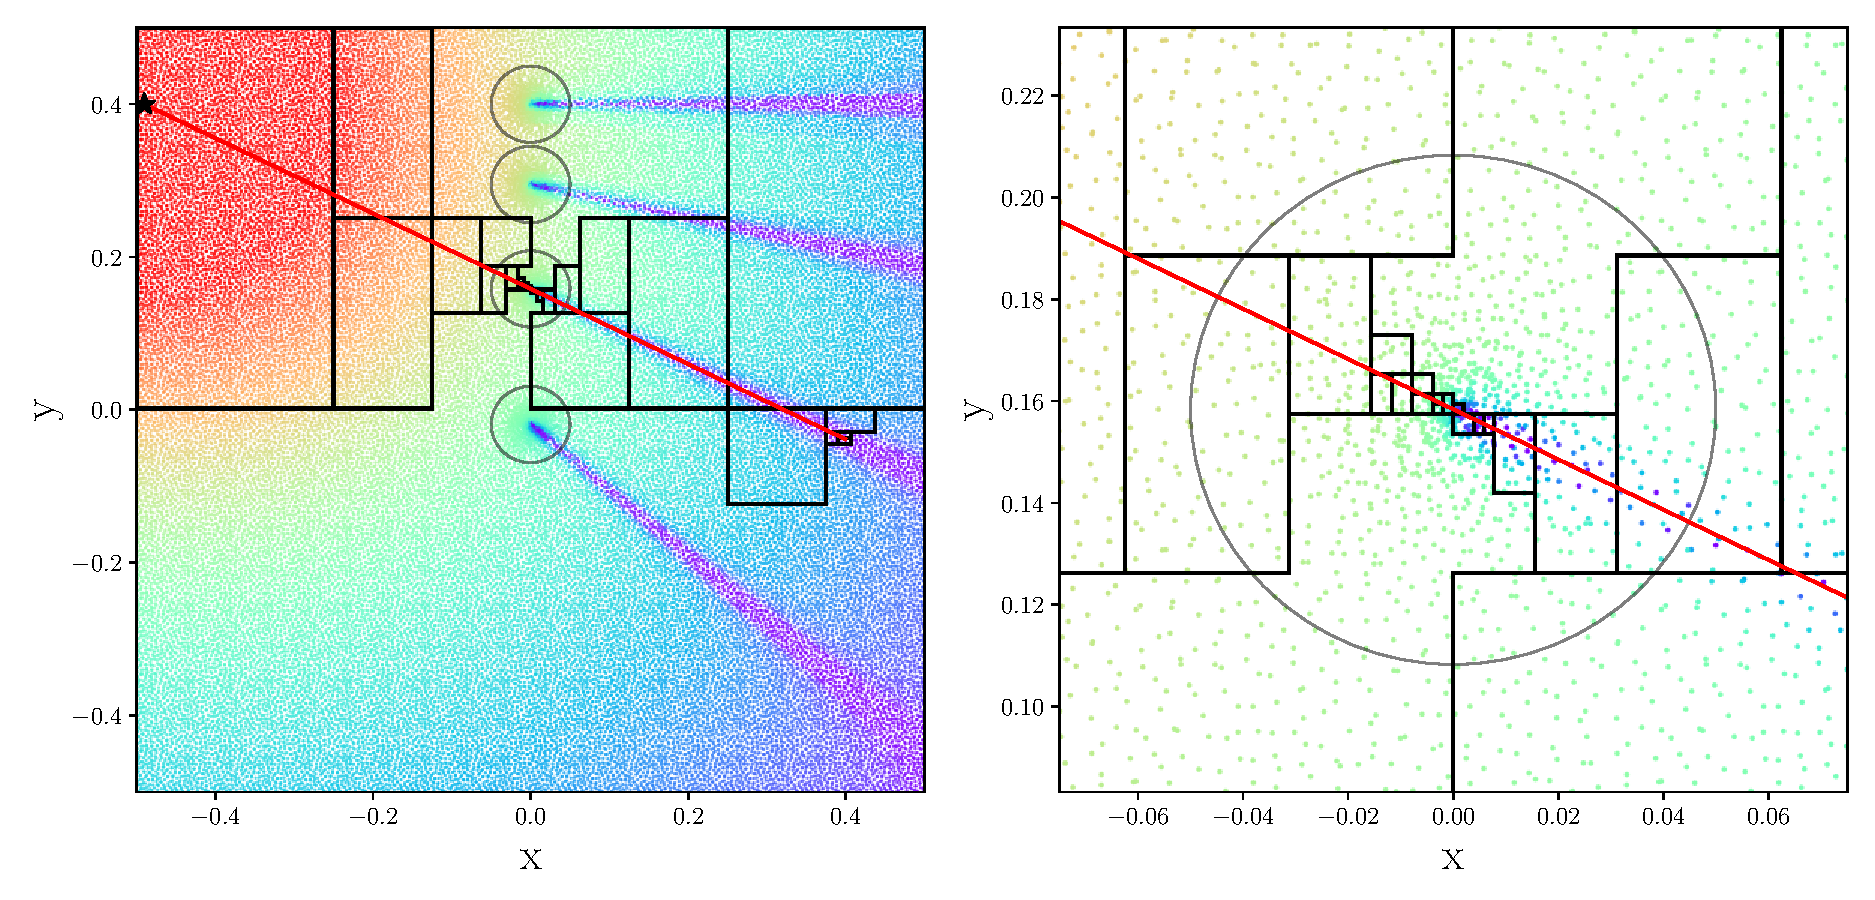
\includegraphics[width=1\linewidth]{Figures/cellplot.pdf}
\caption{}
\label{fig:cellplot}
\end{figure*}
They are centred on the $x$ and $z$ axis with $y$ coordinates given by
\begin{equation}
y_i = 0.75 - 1.3^{-(4-i)},
\end{equation}
where $i$ runs from zero to three. The radiation source, denoted by the black 
star in Figure \ref{fig:cellplot}, is located at $x=0.49$, $y=y_0$ and $z=0$. 
The total number of particles in the IC is $N=4111624$.

\subsubsection{Refinement Criteria}
The effects of the refinement criteria on accuracy and cost in this test were 
analyzed similarly to the data plotted for the Sinusoidally Perturbed glass IC 
test in Figure \ref{fig:refcrit}. The main addition to Figure \ref{fig:isosph} 
is the subset of particles in shadow has its RMS fractional error plotted 
separately to probe the refinement criteria's performance in the optically 
thick regime.
\begin{figure}
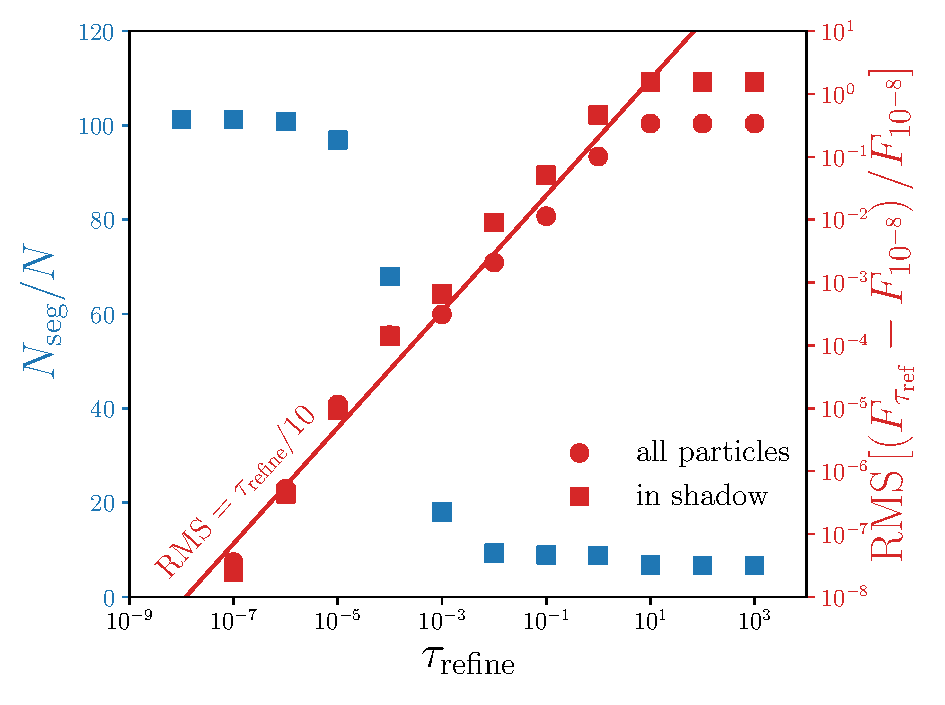
\includegraphics[width=1\linewidth]{Figures/isothermal_spheres.pdf}
\caption{}
\label{fig:isosph}
\end{figure}
Again, $\tr=0.1$ achieves an RMS fractional error of 1\% with very 
little cost. However, when only considering particles in shadow the same 
refinement criteria produces almost an order of magnitude more error at about 
8\%. Decreasing the refinement criteria by an order of magnitude to 
$\tr=0.01$ predictably decreases the RMS fractional error on particles in 
shadow to 1\% with a negligible cost increase from $\tr=0.1$. 

The $\rm{RMS}=\tr$ and $\rm{RMS}=\tr/10$ lines are again plotted in Figure 
\ref{fig:isosph}. For the most part the RMS fractional error is contained 
between these lines, with only two of the in-shadow points at $\tr=1\e{-5}$ 
and $1\e{-4}$,  and one of the all particle points at  $\tr=1\e{-4}$ sitting 
ever so slightly above the $\rm{RMS}=\tr$ line. Again, but now in a more 
difficult test when compared to the sinusoidally perturbed glass IC, Equation 
\ref{eqn:reffrac} proves to accurate in predicting that the maximum allowable 
error in flux per ray segment should be less than and proportional to $\tr$
despite only technically being valid for small $\tau$. In most cases we 
believe \acro{} should perform better as Equation \ref{eqn:reffrac} is just a 
reliable upper bound.

\comment{Wadsley: What about work we did for absolute errors? I'd like at 
least a comment with quantitative error numbers and preferably a plot too. 
Grond: I'll make this for my thesis ASAP and put it here after.}

\subsection{\strom{} Sphere Test}
\subsubsection{\strom{} Sphere Theory}
The \strom{} sphere is a theoretical ionized sphere of gas first discussed by 
Bengt \strom{} in 1938 \citep{stromgren39} as a model of regions around hot, 
young stars. The theoretical initial conditions consist of a cloud neutral 
hydrogen gas with an ionizing source of radiation at its centre. As photons 
from the source ionize the hydrogen, the optical depth of the gas decreases 
and so the ionizing photons are able to travel further and further from the 
source creating an ionization front. As the front moves radially outward from 
the source a radius is reached where the ionization rate equals the 
recombination rate. At this point, the front reaches equilibrium and stops 
creating a stable sphere of ionized hydrogen. The \strom{} sphere test has 
become a common code test in RT methods papers \citep{pawlikSchaye08,
pawlikSchaye11, petkovaSpringel11} and comparison papers \citep{ilievEt06, 
ilievEt09}, as it it is a simple test of a method's ability to resolve 
ionization fronts and achieve equilibrium behaviour.

The equilibrium radius or \strom{} radius, $R_S$, is the radius at which the 
ionization and recombination rates are equal. This radius can be solved for by 
setting the two rates equal producing \citep[e.g.][]{tielens05}
\begin{equation}
R_S = \left(\frac{3}{4\pi}\frac{\dot{N}_\gamma}{\alpha n^2_{H}}\right)^{1/3},
\end{equation}
where $\dot{N}_\gamma$ is the source luminosity in photons per second, 
$\alpha$ is the recombination rate and $n^2_H$ is the hydrogen number density. 
One can also solve for the radius as a function of time 
\citep[e.g.][]{spitzer78},
\begin{equation}
R(t) = R_S\left[1-\exp\left(t/t_{\rm rec}\right)\right]^{1/3}
\end{equation}
where $t_{\rm rec = 1/{n_H \alpha}}$ is the recombination time of the 
gas. The above derivation assumes a ``sharp'' ionization front, meaning the 
transition from ionized to neutral hydrogen is across an infinitesimally small 
region. In practice, the transition region is small compared to the size of 
the ionized region, but there is structure interior to the \strom{} radius 
that is not accounted for by simply solving for the equilibrium radius. In 
order to solve for the non-sharp ionization front we must consider the 
hydrogen ionization equation
\begin{equation}\label{eqn:hion}
\frac{\partial n_{\rm HII}}{\partial t} = c \sigma n_{\rm HI} n_{\gamma} - 
\alpha n_{\rm e} n_{\rm HII},
\end{equation}
where $n_x$ is the number density of species $x$, HI and HII are neutral 
and ionized hydrogen respectively, $\gamma$ is photons, $\sigma$ is the 
ionization cross section, c is the speed of light and $\alpha$ is the 
recombination rate. Note that we have omitted collisional ionization in 
Equation \ref{eqn:hion} as it is not included in further testing, however it 
should be included in general. By integrating the ionization equation and the 
flux equation with absorption (Equation \ref{eqn:simpflux}), we get a solution 
for HI/HII as a function of radius and as a function of time 
\citep{osterbrockFerland2006}. In the following tests, we include both 
theoretical sharp front solution and non-sharp front solutions from the 
\cite{ilievEt06} comparison paper to compare to our results as well as 
mimicking their initial conditions.

\subsubsection{The Isothermal \strom{} Sphere}
\begin{figure}
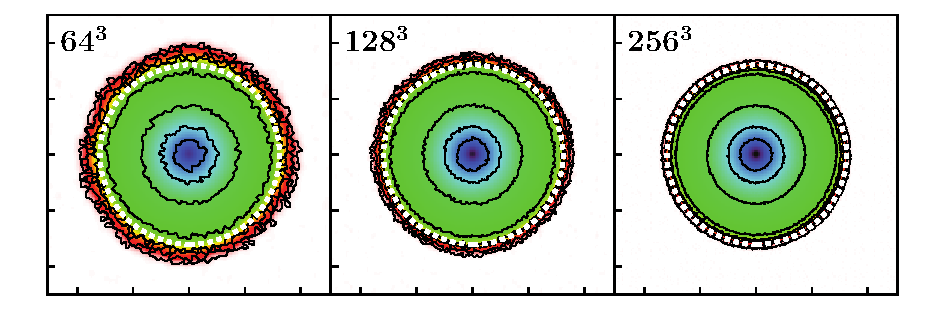
\includegraphics[width=1\linewidth]{Figures/strom_slice_iso_030.pdf}
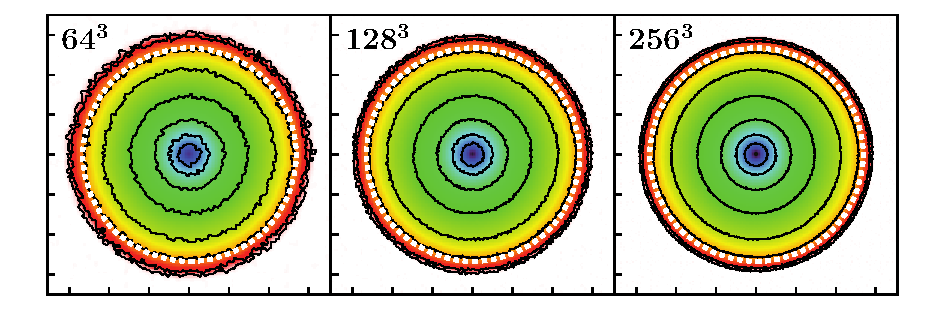
\includegraphics[width=1\linewidth]{Figures/strom_slice_iso_500.pdf}
\caption{}
\label{fig:stromslice}
\end{figure}
In the simplest case, the ionizing source is assumed to emit monochromatic 
photons at 13.6 eV, meaning the gas is ionized but not heated. The gas is not 
allowed to cool, meaning the gas is isothermal. For this reason we will refer 
to this case as the Isothermal \strom{} Sphere. The medium is initially 
neutral with a temperature of $T=10^4$ K and a density of $n_{\rm HI} = 
10^{-3}$ $\rm cm^{-3}$. An ionizing source is turned on at $t=0$ and emits at 
a rate of $\dot{N}_\gamma = 5 \times 10^{48}$ photons $s^{-1}$. We use an 
ionization cross section of $\sigma = 6.3 \times 10^{-18}$ $\rm cm^{-2}$ and a 
recombination rate of $\alpha = 2.59 \times 10^{-13}$ $\rm cm^{-3}$ $\rm 
s^{-1}$, typical of $10^4$ K gas. These values yield a \strom{} radius of 
$R_S = 5.38$ kpc and a recombination time of $t_{rec} \approx  125$ Myr. 

We note that \cite{ilievEt06} uses a 6.6 kpc cube which only contains a single
quadrant of the \strom sphere for their testing. We have opted to use an 16 
kpc cube, increasing the maximum front radius to 8 kpc to avoid any edge 
effects, as the sphere gets close to the edge of the box for some codes in 
their paper. In order to aid comparison, we still normalize radius values to 
6.6 kpc, as is done in \cite{ilievEt06}. As well, we have not imposed a floor 
on the HII fraction of 0.001, as has been done in their paper. As the 
resolution used in the \cite{ilievEt06} comparison paper was never 
specifically given, we have opted to run the test with $N = 64^3$, $128^3$ and 
$256^3$ particles to represent the \textit{entire} sphere. These resolutions 
correspond to single quadrant resolutions of $N=32^3$, $64^3$ and $128^3$ in 
\cite{ilievEt06}. Varying the number of particles also allows us to have a 
look at how \acro{} converges with resolution. We have run our \strom{} sphere 
tests with fixed accuracy parameters of $\theta_{\rm open} = 0.75$, 
$\tau_{\rm ref} = 0.1$.

Figure \ref{fig:stromslice} is a slice through the $z$-plane of the 
simulation. The colour map corresponds to neutral fraction. The contour 
levels and colour map have been chosen to closely mimick Figure 6 in both 
\cite{pawlikSchaye08} and \cite{pawlikSchaye11}. We have done this to 
highlight a main benefit ray tracers like \acro{} have over photon packet 
propagation methods such as TRAPHIC - isotropy. At the same $N=64^3$ particle 
resolution \acro{} is more isotropically symmetric than TRAPHIC, even with 
their use of monte-carlo resampling. Furthermore, \acro{} outperforms TRAPHIC 
in this aspect even at early times (top panels in Figure 
\ref{fig:stromslice}). Here the interior of the \strom{} sphere is represented 
by 3.3 times fewer particles than late time spheres in equilibrium plotted in 
the TRAPHIC papers (in this paper these are in the top panels of Figure 
\ref{fig:stromslice}).

\begin{figure*}
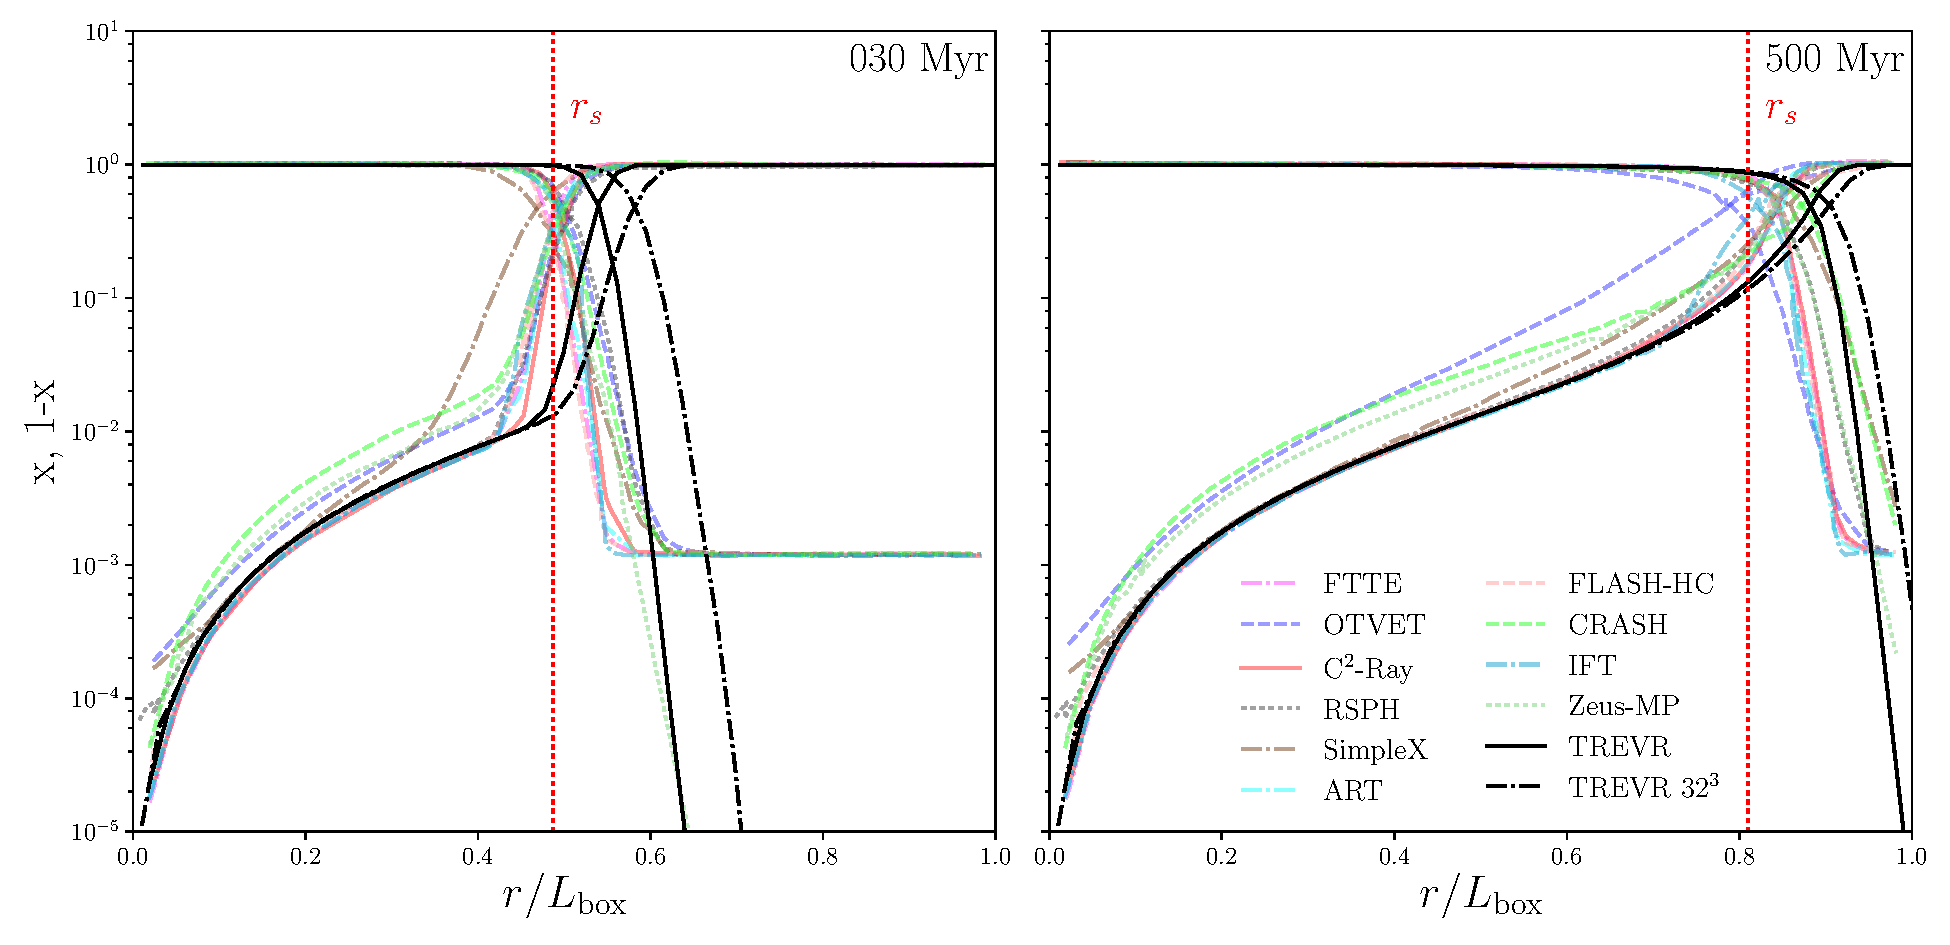
\includegraphics[width=0.95\linewidth]{Figures/strom_iso_fraction.pdf}
\caption{}
\label{fig:stromiso}
\end{figure*}
Figure \ref{fig:stromiso} is a plot of neutral/ionization fraction as a 
function radius from the \strom{} sphere centre. The sharp \strom{} radius is 
plotted as well as non-sharp solutions from all codes presented in Figure 8 
of \cite{ilievEt06}. \acro{} tends to over-ionize at lower resolutions, but 
recreates the ionization profile quite well overall. At 30 Myr we converge 
with resolution to the sharp solution. At 500 Myr we converge to the non-sharp 
numerical solutions, which also over-ionize relative to the sharp solution at 
late times. Overall, the two higher resolution solutions are within the 
scatter of the non-sharp solutions of the codes presented in \cite{ilievEt06}. 
It is interesting to not that the magnitude of over-ionization is related to 
resolution. We suspect the cause of over-ionization is \comment{Grond: What 
exactly do we want to say here?}.

\subsubsection{The Non-Isothermal \strom Sphere}
The above test assumed the hydrogen gas was isothermal and that all incident 
photons had the same energy. In reality, photons range across many wavelengths 
with differing cross-sections at each wavelength. As well, absorption 
typically causes heating, which effects among many gas properties, 
recombination rate.

We rerun the \strom sphere test, but this time the incident photons are 
assumed to be from a black body with temperature $10^5$ K. The cross section 
is now an integrated cross section, obtained by integrating the cross section 
as a function of wavelength between 13.6 eV and 29.65 eV, which gives $\sigma 
= 1.63 \times 10^{-18}$ $\rm cm^{-2}$. The gas has an initial temperature of 
100 K and the recombination rate is a function of temperature set by
\begin{equation}
\alpha(T) = 2.59 \times 10^{-13} \left( \frac{T}{10^4 \hspace{5pt} K}\right)^
{-0.7} \hspace{5pt} cm^{-3} \hspace{5pt} s^{-1}
\end{equation}
to match \cite{petkovaSpringel09}. This test includes heating due to 
absorption and cooling due to recombination $\Delta_r$, collisional 
ionization $\Delta_{ci}$, line cooling $\delta_l$ and Bremsstrahlung 
radiation $\Delta_B$. The rates are taken from \cite{cen92} in order to
match \cite{petkovaSpringel09}.

\begin{figure*}
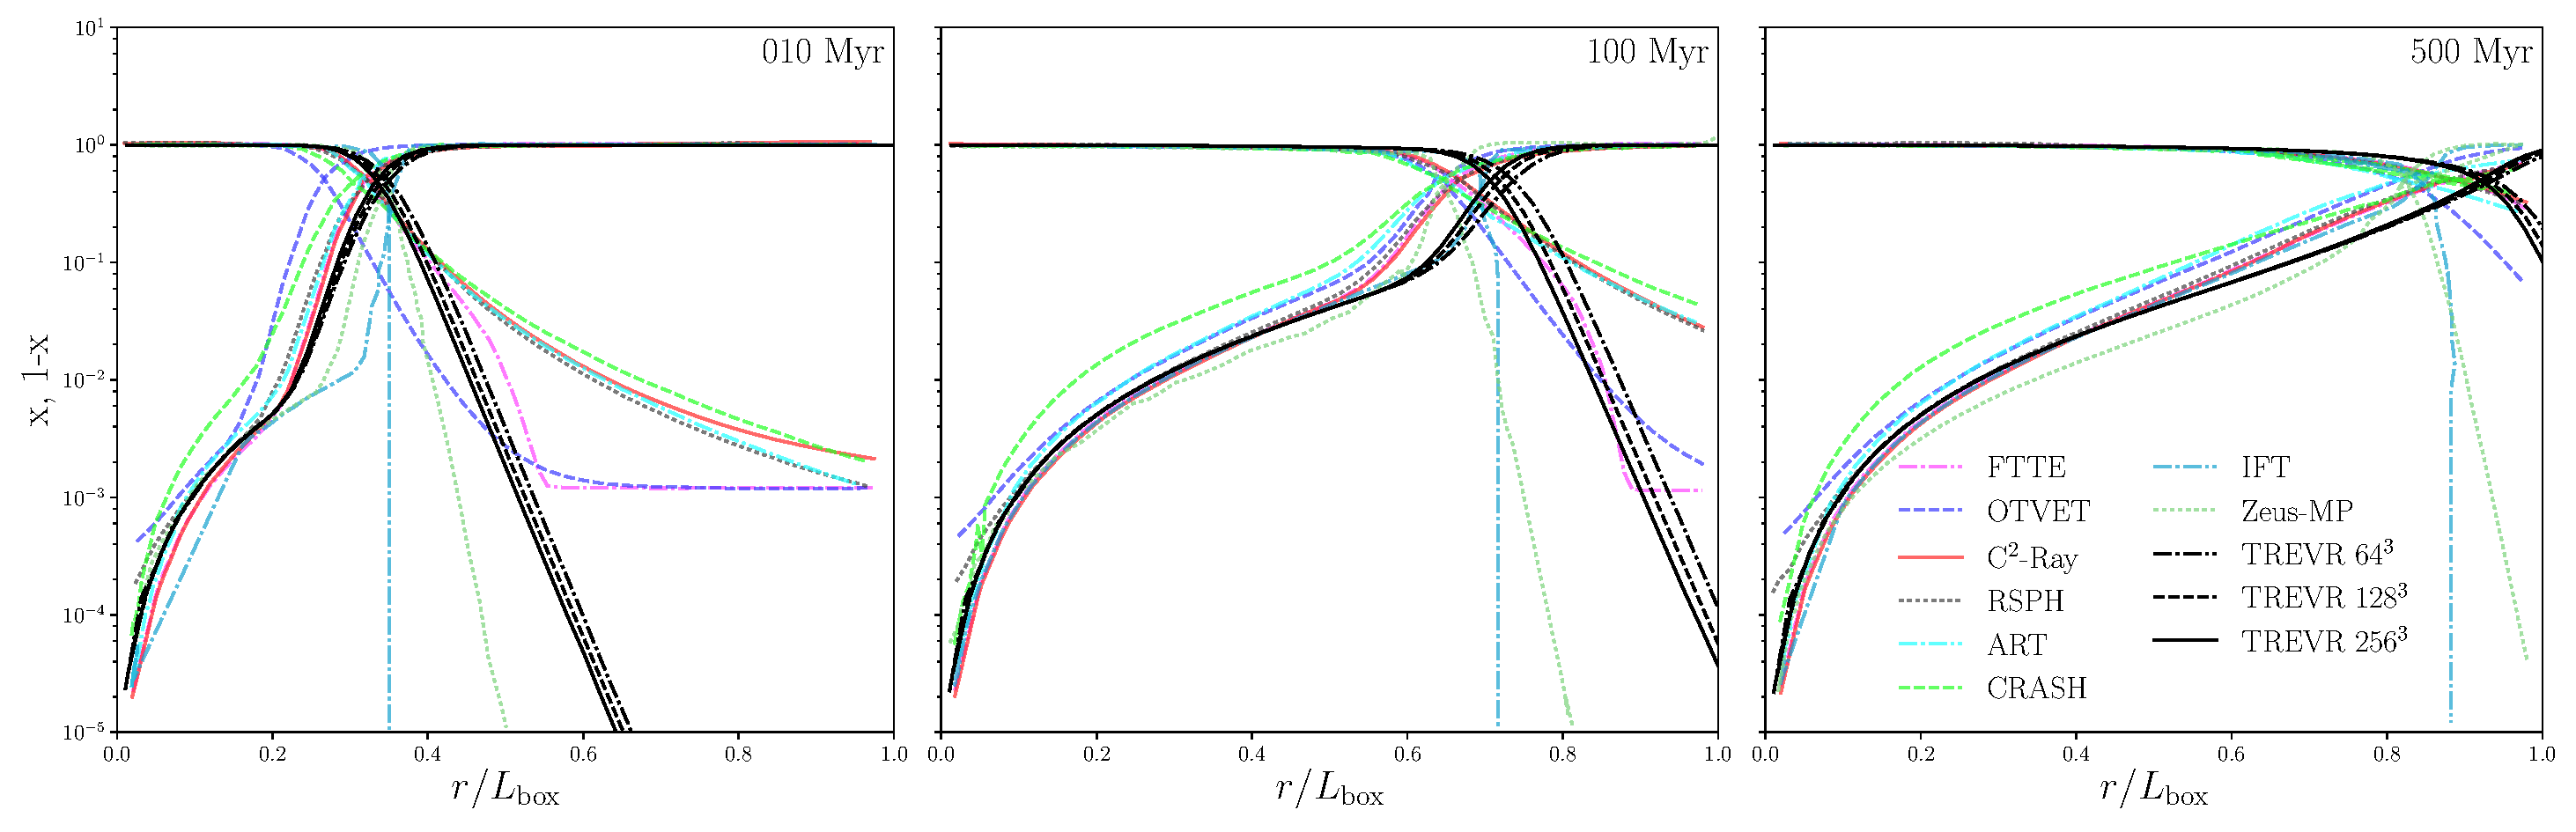
\includegraphics[width=0.95\linewidth]{Figures/strom_fraction.pdf}
\caption{}
\label{fig:stromtherm}
\end{figure*}
\begin{figure*}
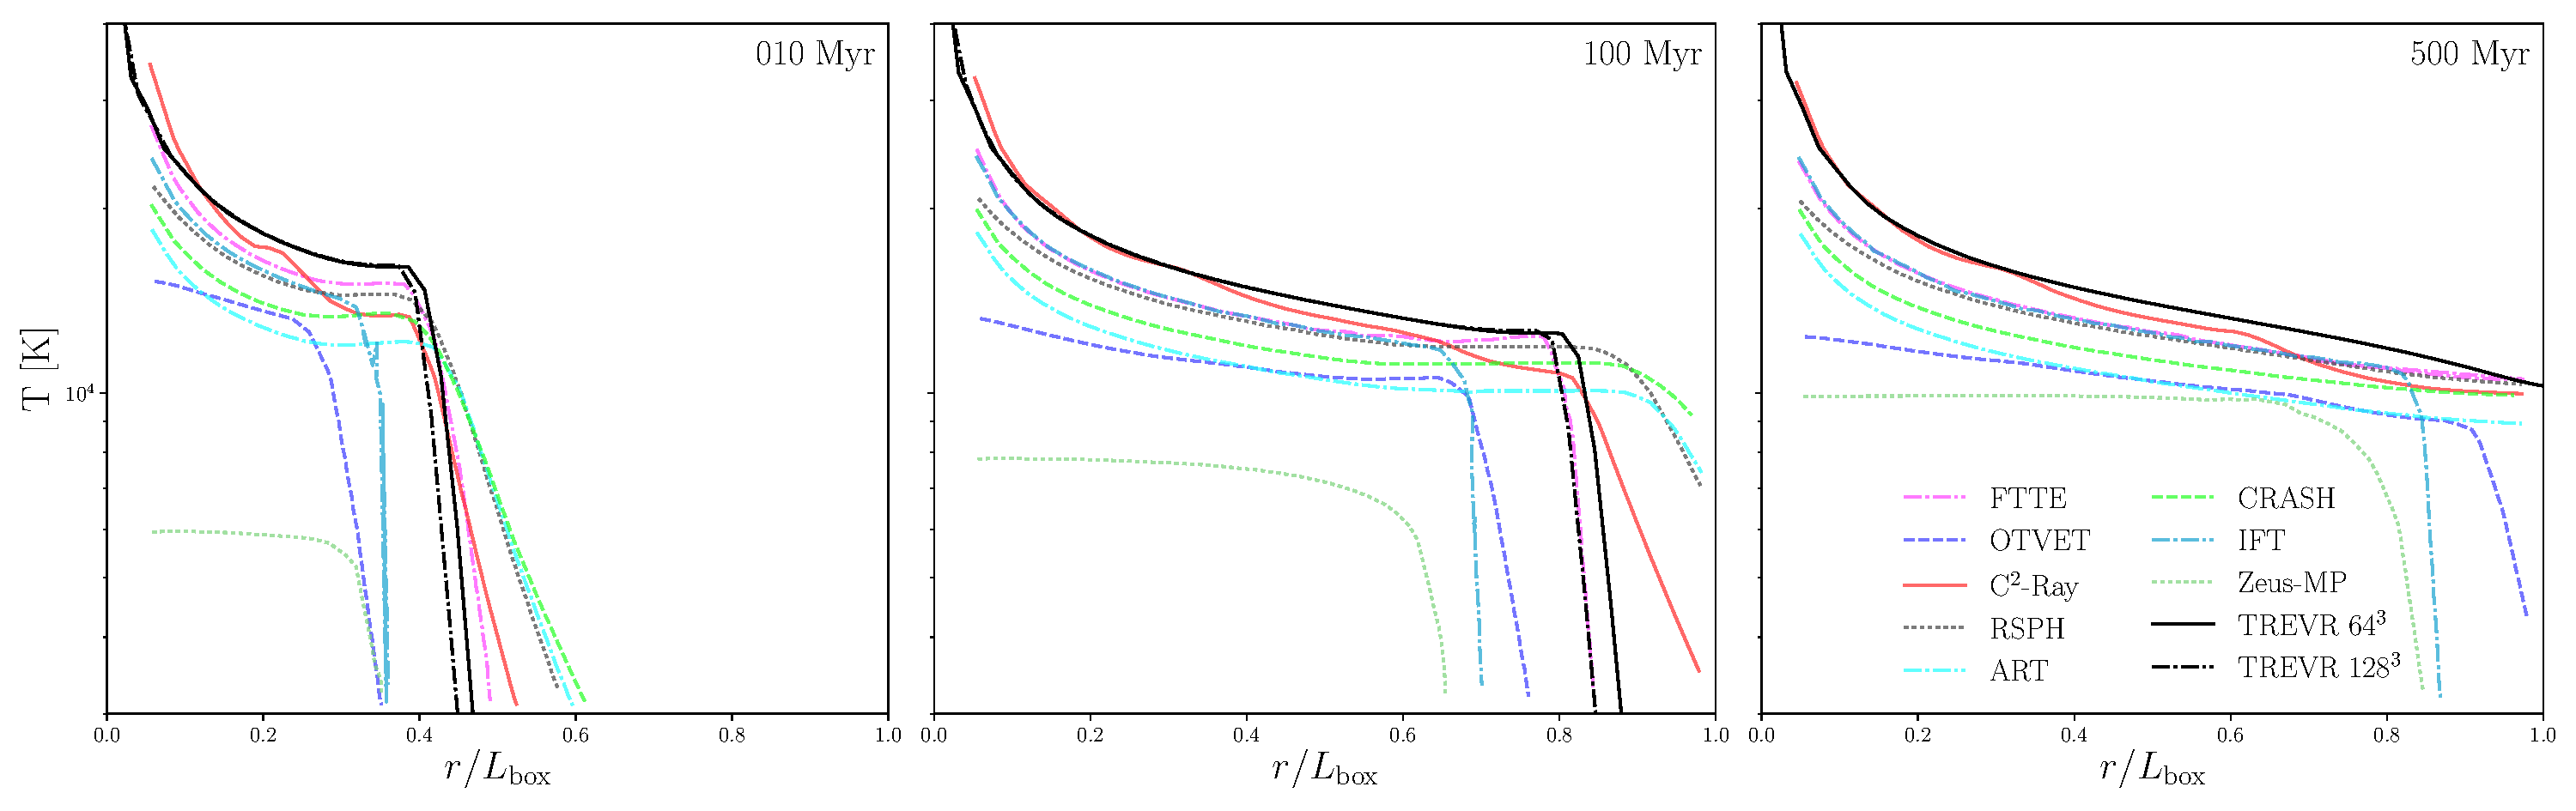
\includegraphics[width=0.95\linewidth]{Figures/strom_temp.pdf}
\caption{}
\label{fig:stromtemp}
\end{figure*}
Figures \ref{fig:stromtherm} and \ref{fig:stromtemp} show the neutral/ionized 
fraction and temperature respectively as a function of radius at $t=$ 10, 100
and 500 Myr. These times represent the fast expansion stage, slowing down 
stage and final \strom{} sphere respectively. We have plotted numerical 
solutions from Figures 16 and 17 in \cite{ilievEt06} for comparison. Again, 
\acro{} recreates these profiles quite well in a qualitative sense. However, 
\acro{} over-ionizes relative to all other solutions at every resolution. We 
believe this is not caused by the \acro{} algorithm specifically, as the 
isothermal test converged with resolution. It could possibly be a result of 
the ionization code and should be addressed in the future \comment{Grond:
Again, exactly what do we want to say here?}. On the other hand, the 
temperature profile lies in the middle of the scatter of the \cite{ilievEt06} 
solutions.


\section{Discussion And Conclusions}\label{sec:disc}
\noindent Best practices
\begin{itemize}
\item what parameters do we suggest based on testing? What one should be 
careful about.
\item specific things we will do wrong?
\end{itemize}

now we have this we can do these things

\noindent Our Niche
\begin{itemize}
\item why are isolated galaxy simulations best right now
\item use in small scale, low source stuff?
\item reionization is bad
\item challenges for the cosmological box use case 
\end{itemize}

\noindent Future Work
\begin{itemize}
\item How to deal with periodicity
\item How to deal with finite speed of light (look back)
\item More optimizations (turning off sources, when to stop tracing a ray)
\item Complex source problem, why it might not be so bad
\end{itemize}

\noindent General Wrap Up
\begin{itemize}
\item Hammer out main points we want to end on (maybe in a list)
\end{itemize}

strict time step

- problem with cosmology (regions of space that generate UV field are 
enormous Gpc, add in background by hand)
- scaling stuff is not specific to gasoline NB=1
- pp (explain it more in context of gasoline)
- cosmo background (stuff merged on sphere)

32*3*N (more hops, resampling)

gasoline has multiple trees (3 trees), future work -> one tree to rule them 
factor of 3

int gasoline section (like sph ray?? how exactly)

For discussion should talk about how this (iso spheres) is hard test -- single 
source.  In more general case if goal is radiation field for chemistry or 
similar errors will tend to cancel in rms

Discussion:   Traffic

$\sim$32 (N+Nvip) packets
- 64 N packet hops per substep 
-- often more even with reduced speed of light b/c must cover c x dt 
(I think Rahmati gave large multiplier)
Will be of order $c_{\rm light}$/$c_{\rm sound}$
Can't really win by doing fewer RT step since just increases the substep 
required
Us $\sim$1000 $N_{\rm sink-active}$ $\sim$10 N per substep, no subcycling needed because on average $N_{\rm sink-active}$ $\sim$ 1/100 N

Discussion should include possible future improvements 
Note: Healpix doesn't change order!
$6N \rightarrow N$


\section*{Acknowledgements}\label{sec:ackn}

%%%%%%%%%%%%%%%%%%%%%%%%%%%%%%

%%%%%%%%%% REFERENCES %%%%%%%%%%

\bibliographystyle{mnras}
\bibliography{references}

%%%%%%%%%%%%%%%%%%%%%%%%%%%%%%

%%%%%%%%%% APPENDICES %%%%%%%%%%

\appendix
\section{Test Initial Conditions}\label{sec:icnd}
\subsection{Sinusoidally Perturbed Glass}
To create our gently varying density distribution for the sink/source scaling 
tests, we modify positions of particles in a glass initial condition by adding 
the sum of 24 sinusoidal modes as in equation \ref{eqn:manfft} below
\begin{equation}\label{eqn:manfft}
\vec{r} = \vec{r}_{\rm 0} + \sum_{i=1}^{24} \frac{1}{275} \sin 
\left( k_{x,i} r_x + k_{y,i} r_y + k_{z,i} r_z + \phi_i\right),
\end{equation}
where $\vec{r_0}$ is the particles initial position in the glass and $\vec{r}$ 
is its perturbed position in the final distribution. The $\vec{k_i}$ and 
$\phi_i$ values are listed in table \ref{tab:modes} for if one wishes to 
reproduce the scaling tests.  
\begin{table}
	\centering
	\caption{Randomly generated $\vec{k}$ and $\phi$ values used in generating 
             a gently varying density distribution.}
	\label{tab:modes}
	\begin{tabular}{llllllll} % four columns, alignment for each
		\hline
		$i$ & $k_{x,i}$ & $k_{y,i}$ & $k_{z,i}$ & $\phi_i$ \\
01 & $-$3.918398 & $+$1.727743 & $-$4.476095 & 0.829776 \\
02 & $-$3.681821 & $-$4.619688 & $+$4.865007 & 3.891157 \\
03 & $-$4.831801 & $+$3.769470 & $+$0.567451 & 3.668730 \\
04 & $-$2.298279 & $+$1.501757 & $+$4.716946 & 1.528348 \\
05 & $-$0.289974 & $-$3.097958 & $+$1.270028 & 4.113001 \\
06 & $+$1.262943 & $-$1.661726 & $-$2.600413 & 4.481799 \\
07 & $+$1.588224 & $+$4.072259 & $+$0.616444 & 2.971965 \\
08 & $-$2.253394 & $-$2.806478 & $+$2.749155 & 0.442241 \\
09 & $-$1.432569 & $+$3.324710 & $+$4.842991 & 2.871989 \\
10 & $+$1.287742 & $-$4.575517 & $-$4.001723 & 1.727810 \\
11 & $+$4.769704 & $+$0.540096 & $-$4.203839 & 5.872117 \\
12 & $-$3.013200 & $-$1.871251 & $-$2.514416 & 1.574008 \\
13 & $-$4.588620 & $+$4.384224 & $+$1.246849 & 1.985715 \\
14 & $-$0.372817 & $+$0.195243 & $+$4.074056 & 6.248739 \\
15 & $-$1.842232 & $+$0.901598 & $-$4.453613 & 6.273336 \\
16 & $+$1.986937 & $-$1.037650 & $+$1.958888 & 2.177783 \\
17 & $-$1.748485 & $-$1.386029 & $+$3.755833 & 0.532604 \\
18 & $+$4.852406 & $-$3.272506 & $+$0.826504 & 5.525470 \\
19 & $+$3.663293 & $-$4.597598 & $-$0.890135 & 4.528870 \\
20 & $-$1.720903 & $+$2.726011 & $+$3.192427 & 3.875610 \\
21 & $+$4.973332 & $+$4.777182 & $-$2.515792 & 0.406737 \\
22 & $+$0.057238 & $-$2.972427 & $-$1.828550 & 4.125258 \\
23 & $+$0.938234 & $-$0.487023 & $-$2.755097 & 1.335299 \\
24 & $+$1.943361 & $+$0.388178 & $-$3.783953 & 4.774938 \\
		\hline
	\end{tabular}
\end{table}
Both gas and star particles have the same density distribution. However, 
the initial glass was flipped for the star particles by reassigning $x$,$y$ 
and $z$ coordinates via
 \begin{equation}
 x_{\rm star} = y_{\rm gas}, \hspace{5pt} y_{\rm star} = z_{\rm gas}, 
 \hspace{5pt} z_{\rm star} = x_{\rm gas},
 \end{equation}
to prevent the particles from occupying the same position in space.
%%%%%%%%%%%%%%%%%%%%%%%%%%%%%%

\bsp
\label{lastpage}
\end{document}

%%%%%%%%%% FIN %%%%%%%%%%
